\documentclass{article}
\usepackage[utf8]{inputenc}
\usepackage{geometry}
\geometry{margin=1in}
\usepackage{amsmath}
\usepackage{amssymb}
\usepackage{amsthm}
\usepackage[ruled,vlined, linesnumbered]{algorithm2e}
\usepackage[english]{babel}
\usepackage[nottoc]{tocbibind}
\usepackage{xcolor}
\usepackage{natbib}
\usepackage{graphicx}
\usepackage{float}
\usepackage{booktabs}
\usepackage{epstopdf}% To incorporate .eps illustrations using PDFLaTeX, etc.
\usepackage{hyperref}
\hypersetup{colorlinks=true, citecolor=black, linkcolor=., urlcolor=cyan}
\newtheorem{theorem}{Theorem}[subsection]
\newtheorem{lemma}{Lemma}[subsection]
\newtheorem{todo}{To Do}
\graphicspath{{fig/}}
\bibliographystyle{unsrt}
\usepackage{appendix}

% Custom commands / shortcuts
\providecommand{\sign}{\textrm{sign}}
\providecommand{\pb}[1]{\textcolor{red}{#1}}
\providecommand{\lam}{\lambda}
\newcommand{\quotes}[1]{``#1''}
\providecommand{\note}[1]{\textcolor{red}{#1}}
\providecommand{\comment}[1]{\textcolor{blue}{#1}}


\title{Adaptive Safe Screening Method for Elastic Net}
\author{Chuyi Wang\\Department of Statistics and Actuarial Sciences\\University of Iowa
  \and
  Patrick Breheny\\Department of Biostatistics\\University of Iowa}
\date{}

\begin{document}

\maketitle




\section{Screening Method}
\subsection{Problem Formulation}

The elastic net problem is the optimization of the following problem:
\begin{equation}
    \label{eq:enet}
    \underset{\beta\in \mathbb{R}^p}{\mathrm{min}}\frac{1}{2}||\boldsymbol y-X\boldsymbol\beta||_2^2+n\alpha\lambda||\boldsymbol\beta||_1+\frac{n(1-\alpha)}{2}\lambda||\boldsymbol\beta||_2^2,
\end{equation}

where $\boldsymbol\beta\in\mathbb{R}^p$ is the coefficient vectors for the $p$ features, $X=[\boldsymbol x_1,\boldsymbol x_2,...,\boldsymbol x_p]\in\mathbb{R}^{n\times p}$ is the feature matrix and $\lambda>0$ is the penalty parameter that controls the size of elastic net penalty. $\alpha\in(0,1)$ is the proportion of Lasso penalty in the elastic net penalty and $1-\alpha$ is the proportion of ridge penalty. A dual form of problem above can be given by (please see appendix for details):

\begin{gather}
        \label{eq:dualtheta}
        \underset{\boldsymbol\theta\in \mathbb{R}^{ n},\boldsymbol\gamma\in\mathbb{R}^p}{\mathrm{max}}g_\lambda(\boldsymbol\theta,\boldsymbol\gamma)\equiv\frac{1}{2}||\boldsymbol y||_2^2-\frac{\lambda^2}{2}\left\Vert\boldsymbol\theta-\frac{\boldsymbol y}{\lambda}\right\Vert_2^2-\frac{\lambda^2}{2}||\boldsymbol\gamma||_2^2\\
        \begin{aligned}s.t.\quad (\boldsymbol\theta,\boldsymbol\gamma)\in \mathcal{F}_\lambda\equiv\{(\boldsymbol\theta,\boldsymbol\gamma):\quad
            &||X^T\boldsymbol\theta-\sqrt{n(1-\alpha)\lambda}\boldsymbol\gamma||_\infty\leq n\alpha\}\nonumber,
        \end{aligned}
\end{gather}

where $\boldsymbol\theta\in \mathbb{R}^{n}$ and $\boldsymbol\gamma\in\mathbb{R}^p$ are the dual variables. The dual problem becomes the minimization of the convex function $g(\boldsymbol\theta,\boldsymbol
\gamma)$ within a convex feasible set $\mathcal{F}_\lambda$. Let $\boldsymbol\beta_\lambda$ denote the solution to the primal problem at penalty parameter value $\lambda$ and $\boldsymbol\theta_{\lambda},\boldsymbol\gamma_\lambda$ denote the corresponding dual solution. The primal solution and dual solution can be connected by

\begin{equation}
    \label{eq:dualprimal}
    \boldsymbol\theta_\lambda=\frac{\boldsymbol y-X\boldsymbol\beta_\lambda}{\lambda},\quad \boldsymbol\gamma_\lambda=\sqrt{\frac{n(1-\alpha)}{\lambda}}\boldsymbol\beta_\lambda,
\end{equation}

and the KKT conditions for the primal problem~\eqref{eq:enet} can be expressed as:

\begin{gather}
    \label{eq:kkt}
    \begin{aligned}&\boldsymbol\beta_{\lambda,j}=0\implies|\boldsymbol x_j^T\boldsymbol\theta_\lambda|\leq n\alpha\\
    & \boldsymbol\beta_{\lambda,j}\neq0\implies  \boldsymbol x_j^T\boldsymbol\theta_\lambda-n(1-\alpha)\boldsymbol\beta_{\lambda,j}=n\alpha\textit{sign}(\boldsymbol\beta_{\lambda,j}).
    \end{aligned}
\end{gather}

for any $j$. Combining \eqref{eq:dualprimal} and \eqref{eq:kkt} we have a trivial closed form solution for the problem at some $\lambda$ values:

\begin{gather}
    \label{eq:lammax}
    \begin{aligned}
        \boldsymbol\beta_\lambda=0\iff \lambda \geq \lambda_{\max}\equiv \max_j \frac{|\boldsymbol x_j^T\boldsymbol y|}{n\alpha}
    \end{aligned}
\end{gather}

Thus, when solving the problems on a grid of $L+1$ decreasing $\lambda$ values: $\lambda_0>\lambda_1>...>\lambda_L>0$, it makes more sense to choose $\lambda_0= \lambda_{\max}$ to take advantage of the known solution. If an algorithm solve the problems sequentially in decreasing order of $\lambda$, then solution at $\lambda_{l-1}$ will be known before solving the problem at $\lambda_l$. In the rest of the paper, we will derive screening method for such a path-wise structure. Also, without loss of generality, we will derive the screening method for the problem at $\lambda_1$ assuming the solution at $\lambda_0$ is known, the same method can be applied to any pair of $\lambda_{l}$ and $\lambda_{l-1}$.

The KKT conditions \eqref{eq:kkt} also say that for any $\lambda$ if 

\begin{equation}
    \label{eq:disc_cond}
    |\boldsymbol x_j^T\boldsymbol\theta_{\lambda}|<n\alpha,
\end{equation}

we can safely conclude $\boldsymbol\beta_{\lambda,j}=0$ and the corresponding $\boldsymbol x_j$ can be discarded for the optimization at $\lambda$. Although the left hand side of \eqref{eq:disc_cond} is unknown at $\lambda_1$ until the solution is obtained at $\lambda_1$, we can use the solution at $\lambda_{0}$ to derive some bound for the left hand side: $T_j(\lambda_{1},\lambda_{0};\boldsymbol\theta_{\lambda_0},\boldsymbol\gamma_{\lambda_0})\geq |\boldsymbol x_j^T\boldsymbol\theta_{\lambda_1}|$ and then if $T_j(\lambda_{1},\lambda_{0};\boldsymbol\theta_{\lambda_0},\boldsymbol\gamma_{\lambda_0})<n\alpha$ we can also safely conclude $\boldsymbol\beta_{\lambda_1,j}=0$. The goal is to find a smaller $T_j(\lambda_{1},\lambda_{0};\boldsymbol\theta_{\lambda_0},\boldsymbol\gamma_{\lambda_0})$ to make more discards. To construct such a bound, we consider the intermediate dual variable:

\begin{gather}
        \label{eq:dualmi}
        (\boldsymbol\theta_{\lambda_1|\lambda_0},\boldsymbol\gamma_{\lambda_1|\lambda_0})\equiv\underset{\boldsymbol\theta\in \mathbb{R}^{ n},\boldsymbol\gamma\in\mathbb{R}^p}{\mathrm{arg\,max}}g_{\lambda_0}(\boldsymbol\theta,\boldsymbol\gamma)\\
        \begin{aligned}s.t.\quad (\boldsymbol\theta,\boldsymbol\gamma)\in \mathcal{F}_{\lambda_1}\nonumber.
        \end{aligned}
\end{gather}

Compared to the origin dual problem \eqref{eq:dualtheta} at $\lambda_0$, the intermediate problem \eqref{eq:dualmi} optimizes the same dual function on a slightly different feasible set, while compared to the intermediate problem, the origin dual problem at $\lambda_1$ optimize a slightly different dual function on the same feasible set. Then we can use the solution $(\boldsymbol\theta_{\lambda_0},\boldsymbol\gamma_{\lambda_0})$ to find a bound such that $(\boldsymbol\theta_{\lambda_1|\lambda_0},\boldsymbol\gamma_{\lambda_1|\lambda_0})\in \mathcal{A}^1(\lambda_1,\lambda_0|\boldsymbol\theta_{\lambda_0},\boldsymbol\gamma_{\lambda_0})$ and after that based on $(\boldsymbol\theta_{\lambda_1|\lambda_0},\boldsymbol\gamma_{\lambda_1|\lambda_0})$ find a second bound such that $(\boldsymbol\theta_{\lambda_1},\boldsymbol\gamma_{\lambda_1})\in \mathcal{A}^2(\lambda_1,\lambda_0|\boldsymbol\theta_{\lambda_1|\lambda_0},\boldsymbol\gamma_{\lambda_1|\lambda_0})$. Last if we find a bound satisfying:

\begin{equation}
    \label{eq:boundbound}
    T_j(\lambda_{1},\lambda_{0};\boldsymbol\theta_{\lambda_0},\boldsymbol\gamma_{\lambda_0})\geq \underset{(\boldsymbol\theta',\boldsymbol\gamma')\in\mathcal{A}^1(\lambda_1,\lambda_0|\boldsymbol\theta_{\lambda_0},\boldsymbol\gamma_{\lambda_0})}{\mathrm{max}}\,\underset{(\boldsymbol\theta,\boldsymbol\gamma)\in\mathcal{A}^2(\lambda_1,\lambda_0|\boldsymbol\theta',\boldsymbol\gamma')}{\mathrm{max}}|\boldsymbol x_j^T\boldsymbol\theta|,
\end{equation}

then it automatically satisfies $T_j(\lambda_{1},\lambda_{0};\boldsymbol\theta_{\lambda_0},\boldsymbol\gamma_{\lambda_0})\geq |\boldsymbol x_j^T\boldsymbol\theta_{\lambda_1}|$ and can be used for screening.

In the case when $\lambda_0=\lambda_{\max}$, a form of the bound $T_j(\lambda_{1},\lambda_{0};\boldsymbol\theta_{\lambda_0},\boldsymbol\gamma_{\lambda_0})$ has been derived in BEDPP for elastic net \citep{Zeng2021}:

\begin{theorem}
    \label{thm:0.1}
    For any $\lambda_1\in(0,\lambda_{\max})$, let $\boldsymbol x_*\equiv\underset{\boldsymbol x_j}{argmax}|\boldsymbol x_j^T\boldsymbol y|$ and $c\equiv \frac{\lambda_{\max}-\lambda_1}{\lambda_{\max}\lambda_1}$, then
    \begin{gather}
        \begin{aligned}
            T_j(\lambda_{1},\lambda_{\max};\boldsymbol\theta_{\lambda_{\max}},\boldsymbol\gamma_{\lambda_{\max}})&=\left|\frac{\lambda_{\max}+\lambda_1}{2\lambda_{\max}\lambda_1}\boldsymbol x_j^T\boldsymbol y-\frac{n\alpha c\lambda_{\max}}{2(||\boldsymbol x_*||_2^2+n(1-\alpha)\lambda_1)}\textit{sign}(\boldsymbol x_j^T\boldsymbol y) \boldsymbol x_j^T\boldsymbol x_*\right|+\\
            &\frac{c}{2}\sqrt{\left(||\boldsymbol x_j||_2^2+n(1-\alpha)\lambda_1\right)\left(||\boldsymbol y||_2^2-\frac{n^2\alpha^2\lambda_{\max}^2}{||\boldsymbol x_*||_2^2+n(1-\alpha)\lambda_1}\right)}.
        \end{aligned}
    \end{gather}
\end{theorem}

Thus, in this paper, we will derive a form of bound for the case when $\lambda_0<\lambda_{\max}$. These two cases together will cover the whole solution path.

\subsection{Origin and Intermediate Dual Variables Bounds}

In this section, we will derive the two bounds $\mathcal{A}^1$ and $\mathcal{A}^2$.

\begin{theorem}
    \label{thm:1.1}
    For any $\lambda_1<\lambda_{0}\in (0,\lambda_{max})$, assuming $(\boldsymbol\theta_{\lambda_0},\boldsymbol\gamma_{\lambda_0})$ is known, $(\boldsymbol\theta_{\lambda_1|\lambda_0},\boldsymbol\gamma_{\lambda_1|\lambda_0})$ is bounded in the set $\mathcal{A}^1(\lambda_1,\lambda_0|\boldsymbol\theta_{\lambda_0},\boldsymbol\gamma_{\lambda_0})$ that is a ball with center and radius
    \begin{gather}
        \begin{aligned}
            \boldsymbol c_1&=\binom{\boldsymbol\theta_{\lambda_0}}{\sqrt{\frac{\lambda_1}{\lambda_0}}\boldsymbol\gamma_{\lambda_0}}\\
            r_1&=\sqrt{c(\lambda_0-\lambda_1)}||\boldsymbol\gamma_{\lambda_0}||_2,
        \end{aligned}
    \end{gather}
\end{theorem}

where $c\equiv\frac{\lambda_0-\lambda_1}{\lambda_0\lambda_1}$. Looking at the form of the dual function \eqref{eq:dualtheta}, $(\boldsymbol\theta_{\lambda_1},\boldsymbol\gamma_{\lambda_1})$ is the projection of $(\frac{\boldsymbol y}{\lambda_1},0)$ onto $\mathcal{F}_{\lambda_1}$, while in the intermediate problem \eqref{eq:dualmi}, $(\boldsymbol\theta_{\lambda_1|\lambda_0},\boldsymbol\gamma_{\lambda_1|\lambda_0})$ is the projection of a different point $(\frac{\boldsymbol y}{\lambda_0},0)$ onto the same set $\mathcal{F}_{\lambda_1}$. Using properties of projection onto a convex set as in the enhanced dual polytope projection (EDPP) \citep{wang2013lasso}, a bound for $(\boldsymbol\theta_{\lambda_1},\boldsymbol\gamma_{\lambda_1})$ can be derived:

\begin{theorem}
    \label{thm:1.2}
    For any $t\geq0$ and $\lambda_1<\lambda_{0}\in (0,\lambda_{max})$, assuming $(\boldsymbol\theta_{\lambda_1|\lambda_0},\boldsymbol\gamma_{\lambda_1|\lambda_0})$ is known, $(\boldsymbol\theta_{\lambda_1},\boldsymbol\gamma_{\lambda_1})$ is bounded in the set $\mathcal{A}^2(\lambda_1,\lambda_0,t|\boldsymbol\theta_{\lambda_1|\lambda_0},\boldsymbol\gamma_{\lambda_1|\lambda_0})$ that is a ball with center and radius
    \begin{gather}
        \begin{aligned}
            \boldsymbol c_2\equiv\binom{\boldsymbol c_2^\theta}{\boldsymbol c_2^\gamma}&=\binom{\frac{1}{2}(\frac{1-t}{\lambda_0}+c)\boldsymbol y+\frac{t+1}{2}\boldsymbol\theta_{\lambda_1|\lambda_0}}{\frac{t+1}{2}\boldsymbol\gamma_{\lambda_0}},\\
            r_2&=\frac{1}{2\lambda_0}\left\Vert\binom{(1-t)(\boldsymbol y-\lambda_0\boldsymbol\theta_{\lambda_1|\lambda_0})+c\lambda_0\boldsymbol y}{(1-t)\lambda_0\boldsymbol\gamma_{\lambda_1|\lambda_0}}\right\Vert_2,
        \end{aligned}
    \end{gather}
    where
    \begin{gather}
        \begin{aligned}
            c&\equiv\frac{\lambda_0-\lambda_1}{\lambda_0\lambda_1}.\\
        \end{aligned}
    \end{gather}
\end{theorem}

Note the result is valid for any $t\geq 0$. Instead of choosing a $t$ at this step as in the EDPP method, we will decide the choice of $t$ in the end of next subsection.

\subsection{Upper Bound in the Combined Bound}


To find the bound in \eqref{eq:boundbound}, we can first consider the problem:

\begin{equation}
    \Tilde{T}_j(\lambda_1,\lambda_0;\boldsymbol\theta',\boldsymbol\gamma')\equiv\underset{(\boldsymbol\theta,\boldsymbol\gamma)\in\mathcal{A}^2(\lambda_1,\lambda_0|\boldsymbol\theta',\boldsymbol\gamma')}{\mathrm{max}}|\boldsymbol x_j^T\boldsymbol\theta|,
\end{equation}

and it can be broken into two sub-problems:

\begin{equation}
    \label{eq:ttilde}
    \Tilde{T}^\xi_j(\lambda_1,\lambda_0;\boldsymbol\theta',\boldsymbol\gamma')\equiv\underset{(\boldsymbol\theta,\boldsymbol\gamma)\in\mathcal{A}^2(\lambda_1,\lambda_0|\boldsymbol\theta',\boldsymbol\gamma')}{\mathrm{max}}\xi \boldsymbol x_j^T\boldsymbol\theta,
\end{equation}

where $\xi\in\{-1,1\}$. The sub-problem \eqref{eq:ttilde} is maximizing a linear function in a ball with center $\boldsymbol c_2$ and radius $r_2$ and the maximum is easy to obtain:

\begin{gather}
    \label{eq:ttildexi}
    \begin{aligned}
        \Tilde{T}^\xi_j(\lambda_1,\lambda_0,t;\boldsymbol\theta',\boldsymbol\gamma')&=\xi\boldsymbol x_j^T\boldsymbol c_2^\theta+||\boldsymbol x_j||_2r_2\\
        &=\xi\left( \frac{1}{2}(\frac{1-t}{\lambda_0}+c)\boldsymbol x_j^T\boldsymbol y+\frac{t+1}{2}\boldsymbol x_j^T\boldsymbol\theta'\right)+\frac{||\boldsymbol x_j||_2|1-t|}{2}\left\Vert\binom{\boldsymbol\theta'-\left(\frac{1}{\lambda_0}+\frac{c}{1-t}\right)\boldsymbol y}{\boldsymbol\gamma'}\right\Vert_2,\\
    \end{aligned}
\end{gather}

where we define $0\cdot||\boldsymbol v_1+\frac{\boldsymbol v_2}{0}||_2\equiv ||\boldsymbol v_2||_2$ for any vector $\boldsymbol v_1,\boldsymbol v_2$. There is an extra parameter $t$, and this bound will be valid for all $t\geq 0$. The maximum of $\Tilde{T}^\xi_j$ on $\mathcal{A}^1$ does not have a simple close form, so we consider an upper bound for it instead.

\begin{theorem}
    \label{thm:2.1}
    For any $\lambda_1<\lambda_{0}\in (0,\lambda_{max})$, $j=1,2,...,p$ and $\xi=-1,1$, assuming $(\boldsymbol\theta_{\lambda_0},\boldsymbol\gamma_{\lambda_0})$ is known, if we define
    \begin{gather}
        \begin{aligned}
            T^\xi_j(\lambda_1,\lambda_0,t;\boldsymbol\theta_{\lambda_0},\boldsymbol\gamma_{\lambda_0})\equiv\frac{\frac{1-t}{\lambda_0}+c}{2}\xi\boldsymbol x_j^T \boldsymbol y+\frac{t+1}{2}\xi \boldsymbol x_j^T \boldsymbol \theta_{\lambda_0}+\frac{t+1+|1-t|}{2}||\boldsymbol x_j||_2\sqrt{c(\lambda_0-\lambda_1)}||\boldsymbol\gamma_{\lambda_0}||_2\\+\frac{||\boldsymbol x_j||_2}{2}\left\Vert\binom{(1-t)\theta_{\lambda_0}-\left(\frac{1-t}{\lambda_0}+c\right)\boldsymbol y}{(1-t)\sqrt{\frac{\lambda_1}{\lambda_0}}\boldsymbol\gamma_{\lambda_0}}\right\Vert_2\\
            %&=\xi \boldsymbol x_j^T \boldsymbol c_1^\theta+||\boldsymbol x_j||_2\left(\sqrt{c(\lambda_0-\lambda_1)}||\boldsymbol c_1^\gamma||_2+\sqrt{1+c(\lambda_0-\lambda_1)}r_1\right).
        \end{aligned}
    \end{gather}
    then $T^\xi_j(\lambda_1,\lambda_0,t;\boldsymbol\theta_{\lambda_0},\boldsymbol\gamma_{\lambda_0})\geq\underset{(\boldsymbol\theta',\boldsymbol\gamma')\in\mathcal{A}^1(\lambda_1,\lambda_0|\boldsymbol\theta_{\lambda_0},\boldsymbol\gamma_{\lambda_0})}{\mathrm{max}}\Tilde{T}^\xi_j(\lambda_1,\lambda_0,t;\boldsymbol\theta',\boldsymbol\gamma')$ for all $t\geq0$.
\end{theorem}

If we define

\begin{gather}
    \begin{aligned}
        \boldsymbol v_1\equiv\binom{\frac{\boldsymbol y}{\lambda_0}-\boldsymbol\theta_{\lambda_0}}{-\sqrt{\frac{\lambda_1}{\lambda_0}}\boldsymbol\gamma_{\lambda_0}}\\
        \boldsymbol v_2\equiv\binom{\frac{\boldsymbol y}{\lambda_0}-\boldsymbol\theta_{\lambda_0}+c\boldsymbol y}{-\sqrt{\frac{\lambda_1}{\lambda_0}}\boldsymbol\gamma_{\lambda_0}}\\
        \tilde{\boldsymbol x}_j\equiv\binom{\xi\boldsymbol x_j}{\boldsymbol 0_p}
    \end{aligned}
\end{gather}

then $T^\xi_j(\lambda_1,\lambda_0,t;\boldsymbol\theta_{\lambda_0},\boldsymbol\gamma_{\lambda_0})$ becomes

\begin{equation}
    \label{eq:txi}
    \xi\boldsymbol x_j^T\theta_{\lambda_0}+\frac{1}{2} \tilde{\boldsymbol x}_j^T(\boldsymbol v_2-t \boldsymbol v_1)+\frac{t+1+|1-t|}{2}||\tilde{\boldsymbol x}_j||_2\sqrt{c(\lambda_0-\lambda_1)}||\boldsymbol\gamma_{\lambda_0}||_2+\frac{1}{2}||\tilde{\boldsymbol x}_j||_2||\boldsymbol v_2-t\boldsymbol v_1||_2.
\end{equation}

Last, we need to choose a $t\geq 0$. An optimal choice will be the $t$ that minimizes $T^\xi_j(\lambda_1,\lambda_0,t;\boldsymbol\theta_{\lambda_0},\boldsymbol\gamma_{\lambda_0})$. This choice results in a complicated form of $t$ and different values of $t$ have to be chosen for different $\boldsymbol x_j$, which may result in additional computation cost that outweighs the gain from screening. Instead, we choose the $t$ that minimizes a simpler objective

\begin{equation}
    \frac{t}{2}||\tilde{\boldsymbol x}_j||_2\sqrt{c(\lambda_0-\lambda_1)}||\boldsymbol\gamma_{\lambda_0}||_2+\frac{1}{2}||\tilde{\boldsymbol x}_j||_2||\boldsymbol v_2-t\boldsymbol v_1||_2.
\end{equation}

The solution will be:

\begin{equation}
    t^*=\begin{cases}
            0,\hfill c(\lambda_0-\lambda_1)||\boldsymbol\gamma_{\lambda_0}||_2^2\geq ||\boldsymbol v_1||^2_2\\
            \left(\frac{\boldsymbol v_1^T\boldsymbol v_2}{||\boldsymbol v_1||_2^2}-\frac{\sqrt{||\boldsymbol v_1||_2^2||\boldsymbol v_2||_2^2-(\boldsymbol v_1^T\boldsymbol v_2)^2}\sqrt{c(\lambda_0-\lambda_1)}||\boldsymbol\gamma_{\lambda_0}||_2}{||\boldsymbol v_1||_2^2\sqrt{||\boldsymbol v_1||_2^2-c(\lambda_0-\lambda_1)||\boldsymbol\gamma_{\lambda_0}||_2^2}}\right)\vee 0,\hfill\quad o.w,
            \end{cases}
\end{equation}

This latter choice won't depend on $j$ and will be close to the optimal choice. If we define $\boldsymbol r_{\lambda_0}\equiv \boldsymbol y-X\boldsymbol\beta_{\lambda_0}$ and $\hat{\boldsymbol y}_{\lambda_0}\equiv X\boldsymbol\beta_{\lambda_0}$, then the results above can be expressed in primal variables:

\begin{gather}
    \begin{aligned}
        T^\xi_j(\lambda_1,\lambda_0,t;\boldsymbol\theta_{\lambda_0},\boldsymbol\gamma_{\lambda_0})=  \left(\frac{1-t}{2\lambda_0}+\frac{c}{2}\right)\xi\boldsymbol x_j^T \boldsymbol y+\frac{t+1}{2\lambda_0}\xi \boldsymbol x_j^T \boldsymbol r_{\lambda_0}+\frac{t+1+|1-t|}{2}||\boldsymbol x_j||_2\sqrt{n(1-\alpha) c^2\lambda_1}||\boldsymbol\beta_{\lambda_0}||_2\\
        +\frac{||\boldsymbol x_j||_2}{2\lambda_0}\sqrt{(1-t)^2||\hat{\boldsymbol y}_{\lambda_0}||_2^2+c^2\lambda_0^2||\boldsymbol y||_2^2+2(1-t)c\lambda_0 \boldsymbol y^T\hat{\boldsymbol y}_{\lambda_0}+(1-t)^2n(1-\alpha)\lambda_1||\boldsymbol\beta_{\lambda_0}||_2^2}
    \end{aligned}
\end{gather}

$T_j(\lambda_1,\lambda_0,t;\boldsymbol\theta_{\lambda_0},\boldsymbol\gamma_{\lambda_0})$ being the maximum of it over $\xi=-1,1$ is

\begin{gather}
    \begin{aligned}
        T_j(\lambda_1,\lambda_0,t;\boldsymbol\theta_{\lambda_0},\boldsymbol\gamma_{\lambda_0})= \left| \left(\frac{1-t}{2\lambda_0}+\frac{c}{2}\right)\boldsymbol x_j^T \boldsymbol y+\frac{t+1}{2\lambda_0} \boldsymbol x_j^T \boldsymbol r_{\lambda_0}\right|+\frac{t+1+|1-t|}{2}||\boldsymbol x_j||_2\sqrt{n(1-\alpha) c^2\lambda_1}||\boldsymbol\beta_{\lambda_0}||_2\\
        +\frac{||\boldsymbol x_j||_2}{2\lambda_0}\sqrt{(1-t)^2||\hat{\boldsymbol y}_{\lambda_0}||_2^2+c^2\lambda_0^2||\boldsymbol y||_2^2+2(1-t)c\lambda_0 \boldsymbol y^T\hat{\boldsymbol y}_{\lambda_0}+(1-t)^2n(1-\alpha)\lambda_1||\boldsymbol\beta_{\lambda_0}||_2^2}
    \end{aligned}
\end{gather}

and $t^*=0$ if

\begin{equation}
    \frac{1}{\lambda_0^2}||\hat{\boldsymbol y}_{\lambda_0}||_2^2+\frac{2\lambda_1-\lambda_0}{\lambda_0\lambda_1}n(1-\alpha)||\boldsymbol\beta_{\lambda_0}||_2^2\leq 0,
\end{equation}

else $t^*=$

\begin{gather}
    \begin{aligned}
        \left(1+\frac{c\lambda_0\boldsymbol y^T\hat{\boldsymbol y}_{\lambda_0}}{||\hat{\boldsymbol y}_{\lambda_0}||_2^2+\lambda_1n(1-\alpha)||\boldsymbol\beta_{\lambda_0}||_2^2}\right\\
        \left-c^2\lambda_0^2\sqrt{\frac{||\boldsymbol y||_2^2\left(||\hat{\boldsymbol y}_{\lambda_0}||_2^2+\lambda_1n(1-\alpha)||\boldsymbol\beta_{\lambda_0}||_2^2\right)-\boldsymbol y^T\hat{\boldsymbol y}_{\lambda_0}}{||\hat{\boldsymbol y}_{\lambda_0}||_2^2+\frac{\lambda_0(2\lambda_1-\lambda_0)}{\lambda_1}n(1-\alpha)||\boldsymbol\beta_{\lambda_0}||_2^2}}
        \frac{||\boldsymbol\beta_{\lambda_0}||_2\sqrt{\lambda_1n(1-\alpha)}}{||\hat{\boldsymbol y}_{\lambda_0}||_2^2+\lambda_1n(1-\alpha)||\boldsymbol\beta_{\lambda_0}||_2^2}\right)\vee0
    \end{aligned}
\end{gather}






\subsection{Sequential Safe Screening Rule}

\section{Experiments}

\subsection{Simulation Study}

We compared our proposed adaptive screening method (Adaptive) to sequential strong rule for elastic net (SSR) in simulated data sets. Active cycling is incorporated into both methods.

The data is simulated from the model: $y=X\beta+0.1\epsilon$. The elements of $X$ and $\epsilon$ are sampled i.i.d from $N(0,1)$. The coefficient vector $\beta$ contains $s$ randomly selected elements equally spaced between $[-\beta_{\max},\beta_{\max}]$, with the remaining $p-s$ elements equal to zero. Each setting is replicated $10$ times to calculate the average time needed to solve the coefficient path. By default we set $p=10,000$, $n=1,000$, $s=20$, $\beta_{\max}=1$, $\alpha=0.9$, $L=100$, $\lambda_{\min}/\lambda_{\max}=0.05$. We consider the following cases where one of the variables above is varying at a time:

\begin{enumerate}
    \item \textbf{Varying proportion of lasso penalty:} $\alpha$ from $0.2$ to $0.999$.
    \item \textbf{Varying signal strength:} $\beta_{\max}$ from $0.05$ to $1$.
    \item \textbf{Varying sample size:} $n$ from $200$ to $10,000$.
    \item \textbf{Varying number of features:} $p$ from $1,000$ to $100,000$.
    \item \textbf{Varying sparsity:} $s$ from $10$ to $300$ while controlling total signal size $\beta_{\max}\times s=20$.
    \item \textbf{Varying number of grid points:}  $L$ from $20$ to $1000$.
    \item \textbf{Varying range of grid:}  $\lambda_{\min}/\lambda_{\max}$ from $0.5$ to $0.002$.
\end{enumerate}

\begin{figure}[h]
    \centering
    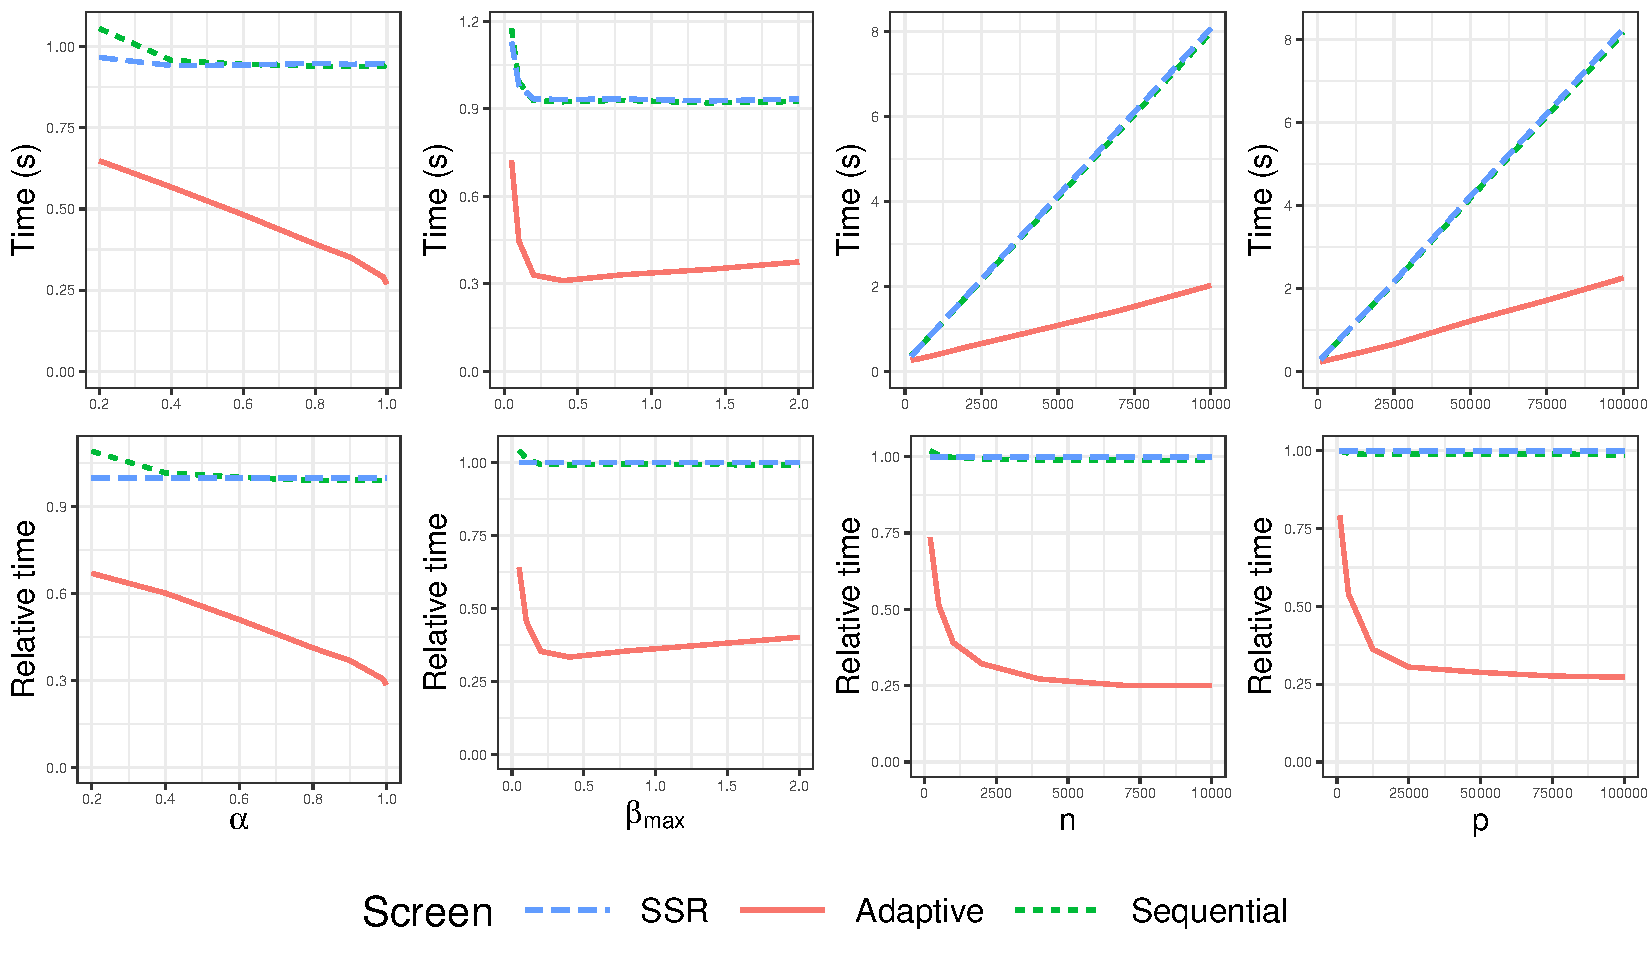
\includegraphics[width=\textwidth]{enet1.pdf}    \caption{Comparing speed of screening methods for lasso model under different settings. Top row: computation time in second. Bottom row: relative computation time compared to SSR. First column: Varying proportion of lasso penalty: $\alpha$. Second column: varying sample size $n$. Third column: varying number of features $p$. Fourth column: varying signal strength $\beta_{\max}$}
    \label{fig:sim1}
\end{figure}

\begin{figure}[h]
    \centering
    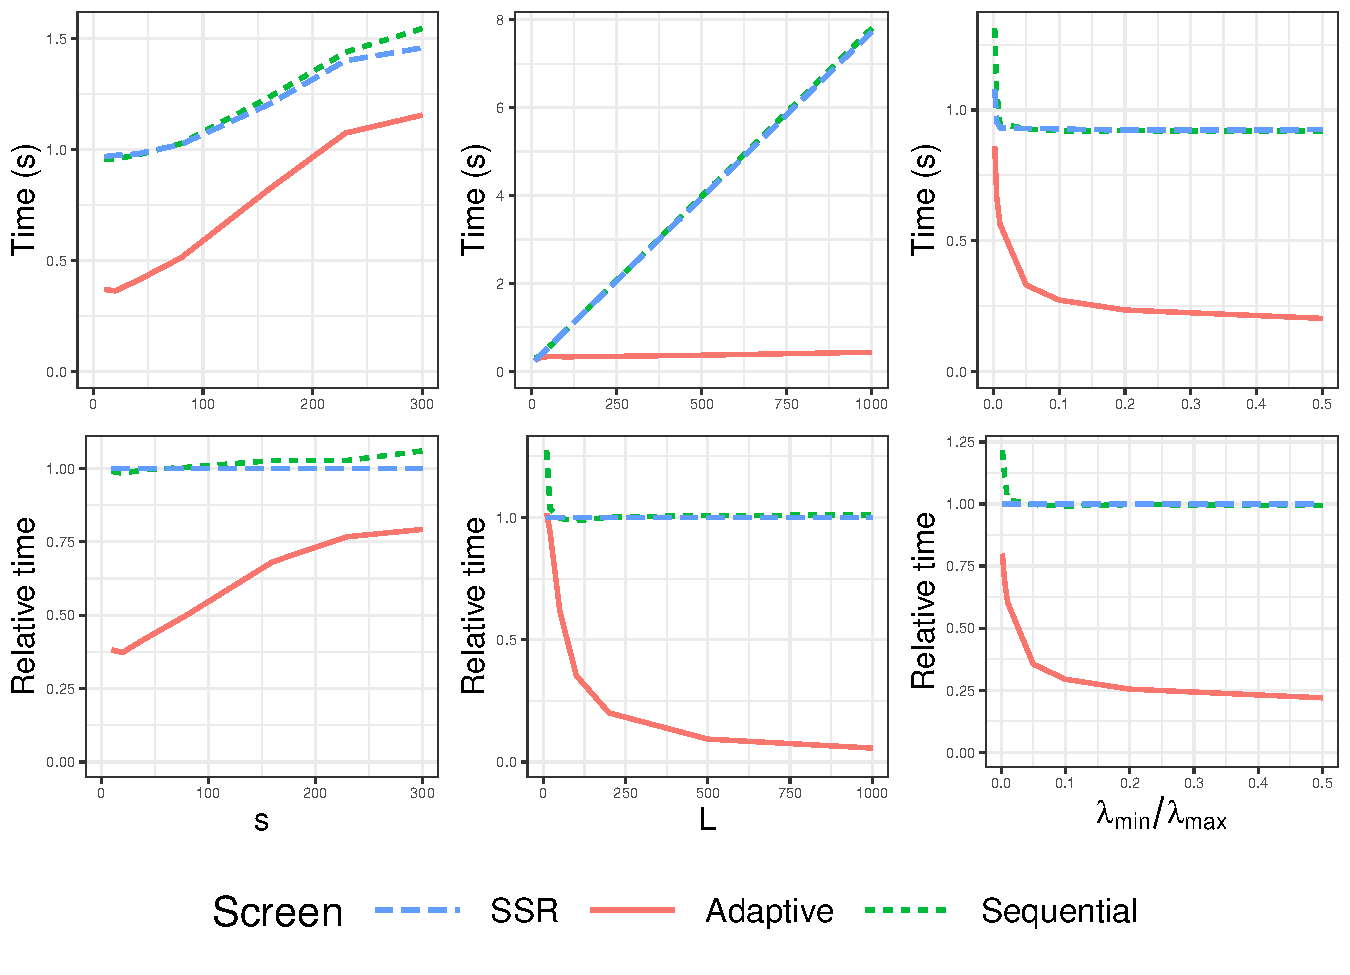
\includegraphics[width=\textwidth]{enet2.pdf}    \caption{Comparing speed of screening methods for lasso model under different settings. Top row: computation time in second. Bottom row: relative computation time compared to SSR. First column: varying sparsity $s$. Second column: Varying number of grid points $L$. Third column: Varying range of grid $\lambda_{\min}/\lambda_{\max}$.}
    \label{fig:sim1}
\end{figure}

\appendix
\appendixpage


\section{Derivation of the Dual Problem}


Introducing 2 new variables $\boldsymbol r\equiv \boldsymbol y-X\boldsymbol\beta$ and $\boldsymbol b\equiv n(1-\alpha)\lambda \boldsymbol\beta$, then the problem \eqref{eq:enet} becomes:

\begin{equation}
    \label{eq:dual+rb}
    \begin{gathered}
    \underset{\boldsymbol\beta\in \mathbb{R}^p}{\mathrm{min}}\frac{1}{2}||\boldsymbol r||_2^2+\frac{1}{2n(1-\alpha)\lambda}||\boldsymbol b||_2^2+n\alpha\lambda||\boldsymbol\beta||_1\\s.t.\quad \boldsymbol r=\boldsymbol y-X\boldsymbol\beta,\quad \boldsymbol b=n(1-\alpha)\lambda \boldsymbol\beta.
\end{gathered}
\end{equation}

Introducing the dual variables $\boldsymbol u\in\mathbb{R}^{n},\boldsymbol w\in\mathbb{R}^p$, the dual problem becomes:

\begin{gather}
    \label{eq:dual+uw}
    \begin{aligned}
        &\underset{\boldsymbol u,\boldsymbol w}{\mathrm{max}}\,\underset{\boldsymbol r,\boldsymbol b}{\mathrm{min}}\,\underset{\boldsymbol\beta}{\mathrm{min}}\,\frac{1}{2}||\boldsymbol r||_2^2+\frac{1}{2n(1-\alpha)\lambda}||\boldsymbol b||_2^2+n\alpha\lambda||\boldsymbol\beta||_1+\boldsymbol u^T(\boldsymbol y-X\boldsymbol\beta-\boldsymbol r)+\boldsymbol w^T\left(\boldsymbol\beta-\frac{\boldsymbol b}{n(1-\alpha)\lambda}\right)\\
        =&\underset{\boldsymbol u,\boldsymbol w}{\mathrm{max}}\,\underset{\boldsymbol r,\boldsymbol b}{\mathrm{min}}\,\underset{\boldsymbol\beta}{\mathrm{min}}\,n\alpha\lambda||\boldsymbol\beta||_1-\boldsymbol u^TX\boldsymbol\beta+\boldsymbol w^T\boldsymbol\beta+\frac{1}{2}||\boldsymbol r||_2^2+\boldsymbol u^T(\boldsymbol y-\boldsymbol r)+\frac{1}{2n(1-\alpha)\lambda}||\boldsymbol b||_2^2-\frac{\boldsymbol w^T\boldsymbol b}{n(1-\alpha)\lambda}
    \end{aligned}    
\end{gather}


Minimizing with respect to $\boldsymbol\beta$, the partial derivative is:

\begin{equation}
    \label{eq:partialbeta}
    \frac{\partial}{\partial\boldsymbol\beta}(\cdot) =-X^T\boldsymbol u+\boldsymbol w+n\alpha\lambda\frac{\partial||\boldsymbol\beta||_1}{\partial\boldsymbol\beta},
\end{equation}

so the minimum is obtained iff $||X^T\boldsymbol u-\boldsymbol w||_\infty\leq n\alpha\lambda,$ and the problem becomes:

\begin{gather}
    \label{eq:dualuw}
    \begin{aligned}
        &\underset{\boldsymbol u,\boldsymbol w}{\mathrm{max}}\,\underset{\boldsymbol r,\boldsymbol b}{\mathrm{min}}\,\frac{1}{2}||\boldsymbol r||_2^2+\boldsymbol u^T(\boldsymbol y-\boldsymbol r)+\frac{1}{2n(1-\alpha)\lambda}||\boldsymbol b||_2^2-\frac{\boldsymbol w^T\boldsymbol b}{n(1-\alpha)\lambda}\\
        =&\underset{\boldsymbol u,\boldsymbol w}{\mathrm{max}}\,\underset{\boldsymbol r,\boldsymbol b}{\mathrm{min}}\,\frac{1}{2}||\boldsymbol r-\boldsymbol u||_2^2+\boldsymbol u^T\boldsymbol y-\frac{1}{2}||\boldsymbol u||_2^2+\frac{1}{2n(1-\alpha)\lambda}||\boldsymbol b-\boldsymbol w||_2^2-\frac{1}{2n(1-\alpha)\lambda}||\boldsymbol w||_2^2\\
        =&\underset{\boldsymbol u,\boldsymbol w}{\mathrm{max}}\,\underset{\boldsymbol r,\boldsymbol b}{\mathrm{min}}\,\frac{1}{2}||\boldsymbol r-\boldsymbol u||_2^2+\frac{1}{2}||\boldsymbol y||_2^2-\frac{1}{2}||\boldsymbol u-\boldsymbol y||_2^2+\frac{1}{2n(1-\alpha)\lambda}||\boldsymbol b-\boldsymbol w||_2^2-\frac{1}{2n(1-\alpha)\lambda}||\boldsymbol w||_2^2\\
        =&\underset{\boldsymbol u,\boldsymbol w}{\mathrm{max}}\,\frac{1}{2}||\boldsymbol y||_2^2-\frac{1}{2}||\boldsymbol u-\boldsymbol y||_2^2-\frac{1}{2n(1-\alpha)\lambda}||\boldsymbol w||_2^2,
    \end{aligned}
\end{gather}

where the minimum is obtained iff $\boldsymbol r=\boldsymbol u$ and $\boldsymbol b=\boldsymbol w$. Let $\boldsymbol\theta\equiv\frac{\boldsymbol u}{\lambda}=\frac{\boldsymbol y-X\boldsymbol\beta}{\lambda}$ and $\boldsymbol\gamma\equiv\frac{\boldsymbol w}{\sqrt{n(1-\alpha)\lambda^3}}=\sqrt{\frac{n(1-\alpha)}{\lambda}}\boldsymbol\beta$ The problem becomes the dual problem in \eqref{eq:dualtheta} and the dual solution and primal solution can be connected by \eqref{eq:dualprimal}.

\section{Proof of Theorem \ref{thm:1.1}}


Considering the second order expansion of $g_{\lambda_0}$ at $(\boldsymbol\theta_{\lambda_0},\boldsymbol\gamma_{\lambda_0})$, $g_{\lambda_0}\left(\boldsymbol\theta_{\lambda_1|\lambda_0},\sqrt{\frac{\lambda_1}{\lambda_0}}\boldsymbol\gamma_{\lambda_1|\lambda_0}\right)$ can be written as

\begin{equation}
    \label{eq:1.1.1}
    g_{\lambda_0}\binom{\boldsymbol\theta_{\lambda_1|\lambda_0}}{\sqrt{\frac{\lambda_1}{\lambda_0}}\boldsymbol\gamma_{\lambda_1|\lambda_0}}=g_{\lambda_0}\binom{\boldsymbol\theta_{\lambda_0}}{\boldsymbol\gamma_{\lambda_0}}+\left\langle\nabla g_{\lambda_0}\binom{\boldsymbol\theta_{\lambda_0}}{\boldsymbol\gamma_{\lambda_0}},\binom{\boldsymbol\theta_{\lambda_1|\lambda_0}}{\sqrt{\frac{\lambda_1}{\lambda_0}}\boldsymbol\gamma_{\lambda_1|\lambda_0}}-\binom{\boldsymbol\theta_{\lambda_0}}{\boldsymbol\gamma_{\lambda_0}}\right\rangle-\frac{\lambda_0^2}{2}\left\Vert\binom{\boldsymbol\theta_{\lambda_1|\lambda_0}}{\sqrt{\frac{\lambda_1}{\lambda_0}}\boldsymbol\gamma_{\lambda_1|\lambda_0}}-\binom{\boldsymbol\theta_{\lambda_0}}{\boldsymbol\gamma_{\lambda_0}}\right\Vert_2^2,
\end{equation}

because $\nabla^2g_{\lambda_0}$ is $-\lambda_0^2$ times the identity matrix. 

First, both $(\boldsymbol\theta_{\lambda_0},\boldsymbol\gamma_{\lambda_0})$ and $\left(\boldsymbol\theta_{\lambda_1|\lambda_0},\sqrt{\frac{\lambda_1}{\lambda_0}}\boldsymbol\gamma_{\lambda_1|\lambda_0}\right)$ are in the convex set $\mathcal{F}_{\lambda_0}$, because

\begin{equation}
    \left\Vert X^T\boldsymbol\theta_{\lambda_1|\lambda_0}-\sqrt{n(1-\alpha)\lambda_0}\sqrt{\frac{\lambda_1}{\lambda_0}}\boldsymbol\gamma_{\lambda_1|\lambda_0}\right\Vert_\infty= \left\Vert X^T\boldsymbol\theta_{\lambda_1|\lambda_0}-\sqrt{n(1-\alpha)\lambda_1}\boldsymbol\gamma_{\lambda_1|\lambda_0}\right\Vert_\infty\leq n\alpha.
\end{equation}

$(\boldsymbol\theta_{\lambda_0},\boldsymbol\gamma_{\lambda_0})$ is the maximizer in the convex set $\mathcal{F}_{\lambda_0}$. That implies that

\begin{equation}
    \label{eq:1.1.2}
    \left\langle\nabla g_{\lambda_0}\binom{\boldsymbol\theta_{\lambda_0}}{\boldsymbol\gamma_{\lambda_0}},\binom{\boldsymbol\theta_{\lambda_1|\lambda_0}}{\sqrt{\frac{\lambda_1}{\lambda_0}}\boldsymbol\gamma_{\lambda_1|\lambda_0}}-\binom{\boldsymbol\theta_{\lambda_0}}{\boldsymbol\gamma_{\lambda_0}}\right\rangle\leq 0.
\end{equation}

Second, by the same argument, both $(\boldsymbol\theta_{\lambda_1|\lambda_0},\boldsymbol\gamma_{\lambda_1|\lambda_0})$ and $\left(\boldsymbol\theta_{\lambda_0},\sqrt{\frac{\lambda_0}{\lambda_1}}\boldsymbol\gamma_{\lambda_0}\right)$ are in the convex set $\mathcal{F}_{\lambda_1}$. Then,

\begin{gather}
    \label{eq:1.1.3}
    \begin{aligned}
        g_{\lambda_0}\binom{\boldsymbol\theta_{\lambda_1|\lambda_0}}{\sqrt{\frac{\lambda_1}{\lambda_0}}\boldsymbol\gamma_{\lambda_1|\lambda_0}}&=\frac{1}{2}||\boldsymbol y||_2^2-\frac{\lambda_0^2}{2}\left\Vert\frac{\boldsymbol y}{\lambda_0}-\boldsymbol\theta_{\lambda_1|\lambda_0}\right\Vert_2^2-\frac{\lambda_1\lambda_0}{2}||\boldsymbol\gamma_{\lambda_1|\lambda_0}||_2^2\\
        &= \frac{1}{2}||\boldsymbol y||_2^2-\frac{\lambda_0^2}{2}\left\Vert\frac{\boldsymbol y}{\lambda_0}-\boldsymbol\theta_{\lambda_1|\lambda_0}\right\Vert_2^2-\frac{\lambda_0^2}{2}||\boldsymbol\gamma_{\lambda_1|\lambda_0}||_2^2+\left(\frac{\lambda_0^2}{2}-\frac{\lambda_1\lambda_0}{2}\right)||\boldsymbol\gamma_{\lambda_1|\lambda_0}||_2^2\\
        &=g_{\lambda_0}\binom{\boldsymbol\theta_{\lambda_1|\lambda_0}}{\boldsymbol\gamma_{\lambda_1|\lambda_0}}+\frac{\lambda_0(\lambda_0-\lambda_1)}{2}||\boldsymbol\gamma_{\lambda_1|\lambda_0}||_2^2\\
        &\geq g_{\lambda_0}\binom{\boldsymbol\theta_{\lambda_0}}{\sqrt{\frac{\lambda_0}{\lambda_1}}\boldsymbol\gamma_{\lambda_0}}+\frac{\lambda_0(\lambda_0-\lambda_1)}{2}||\boldsymbol\gamma_{\lambda_1|\lambda_0}||_2^2\\
        &=g_{\lambda_0}\binom{\boldsymbol\theta_{\lambda_0}}{\boldsymbol\gamma_{\lambda_0}}-\frac{\lambda_0^2(\lambda_0-\lambda_1)}{2\lambda_1}||\boldsymbol\gamma_{\lambda_0}||_2^2+\frac{\lambda_0(\lambda_0-\lambda_1)}{2}||\boldsymbol\gamma_{\lambda_1|\lambda_0}||_2^2,
    \end{aligned}
\end{gather}

where the inequality is due to the fact that $(\boldsymbol\theta_{\lambda_1},\boldsymbol\gamma_{\lambda_1})$ is the maximizer in $\mathcal{F}_{\lambda_1}$. Combining \eqref{eq:1.1.1}, \eqref{eq:1.1.2} and \eqref{eq:1.1.3} we have:

\begin{gather}
    \begin{aligned}
        &\left\Vert\binom{\boldsymbol\theta_{\lambda_1|\lambda_0}}{\sqrt{\frac{\lambda_1}{\lambda_0}}\boldsymbol\gamma_{\lambda_1|\lambda_0}}-\binom{\boldsymbol\theta_{\lambda_0}}{\boldsymbol\gamma_{\lambda_0}}\right\Vert_2^2\leq c\lambda_0||\boldsymbol\gamma_{\lambda_0}||_2^2-c\lambda_1||\boldsymbol\gamma_{\lambda_1|\lambda_0}||_2^2,
    \end{aligned}
\end{gather}

and rearranging the terms yields the result in Theorem \ref{thm:1.1}:

\begin{gather}
    \begin{aligned}
        ||\boldsymbol\theta_{\lambda_1|\lambda_0}-\boldsymbol\theta_{\lambda_0}||_2^2&\leq c\lambda_0||\boldsymbol\gamma_{\lambda_0}||_2^2-c\lambda_1||\boldsymbol\gamma_{\lambda_1|\lambda_0}||_2^2-\left\Vert\sqrt{\frac{\lambda_1}{\lambda_0}}\boldsymbol\gamma_{\lambda_1|\lambda_0}-\boldsymbol\gamma_{\lambda_0}\right\Vert_2^2\\
        &=c\lambda_0||\boldsymbol\gamma_{\lambda_0}||_2^2-c\lambda_1||\boldsymbol\gamma_{\lambda_1|\lambda_0}||_2^2-\frac{\lambda_1}{\lambda_0}||\boldsymbol\gamma_{\lambda_1|\lambda_0}||_2^2+2\sqrt{\frac{\lambda_1}{\lambda_0}}\boldsymbol\gamma_{\lambda_0}^T\boldsymbol\gamma_{\lambda_1|\lambda_0}-||\boldsymbol\gamma_{\lambda_0}||_2^2\\
        &=-||\boldsymbol\gamma_{\lambda_1|\lambda_0}||_2^2+2\sqrt{\frac{\lambda_1}{\lambda_0}}\boldsymbol\gamma_{\lambda_0}^T\gamma_{\lambda_1|\lambda_0}+(c\lambda_0-1)||\boldsymbol\gamma_{\lambda_0}||_2^2\\
        &=-\left\Vert\boldsymbol\gamma_{\lambda_1|\lambda_0}-\sqrt{\frac{\lambda_1}{\lambda_0}}\boldsymbol\gamma_{\lambda_0}\right\Vert_2^2+c(\lambda_0-\lambda_1)||\boldsymbol\gamma_{\lambda_0}||_2^2\\
        \implies \left\Vert\binom{\boldsymbol\theta_{\lambda_1|\lambda_0}}{\boldsymbol\gamma_{\lambda_1|\lambda_0}}-\binom{\boldsymbol\theta_{\lambda_0}}{\sqrt{\frac{\lambda_1}{\lambda_0}}\boldsymbol\gamma_{\lambda_0}}\right\Vert_2^2&\leq c(\lambda_0-\lambda_1)||\boldsymbol\gamma_{\lambda_0}||_2^2.
    \end{aligned}
\end{gather}

\section{Proof of Theorem \ref{thm:1.2}}

From a geometric aspect, the dual problem \eqref{eq:dualtheta} is minimizing an $L_2$ distance, or in other word , finding a projection. $(\boldsymbol \theta_{\lambda_1|\lambda_0},\boldsymbol \gamma_{\lambda_1|\lambda_0})$ is the projection of $(\frac{\boldsymbol y}{\lambda_0},\boldsymbol0)$ onto $\mathcal{F}_{\lambda_1}$ while $(\boldsymbol \theta_{\lambda_1},\boldsymbol \gamma_{\lambda_1})$ is the projection of $(\frac{\boldsymbol y}{\lambda_1},\boldsymbol0)$ onto the same set $\mathcal{F}_{\lambda_1}$. $\mathcal{F}_{\lambda_1}$ is a nonempty closed convex set. We define

\begin{gather}
    \label{eq:1.2.1}
    \begin{aligned}
        \boldsymbol v_1\equiv\binom{\frac{\boldsymbol y}{\lambda_0}-\boldsymbol \theta_{\lambda_1|\lambda_0}}{-\boldsymbol \gamma_{\lambda_1|\lambda_0}},\\
        \boldsymbol v_2\equiv \binom{\frac{\boldsymbol y}{\lambda_1}-\boldsymbol \theta_{\lambda_1|\lambda_0}}{-\boldsymbol \gamma_{\lambda_1|\lambda_0}}.
    \end{aligned}
\end{gather}

First, we have the idea of projections of rays, stated as the following

\begin{lemma}
    \citep{Bauschke2011}
    Let $\mathcal{C}$ be a nonempty closed convex subset of a Hilbert space $\mathcal{H}$. For any $\boldsymbol w\in\mathcal{H}$ , let $P_{\mathcal{C}}(\boldsymbol w)$ be the projection of $\boldsymbol w$ onto $\mathcal{C}$. Then for any $\boldsymbol w\in\mathcal{H}$ and $t\geq 0$,
    \begin{equation}
        P_{\mathcal{C}}\left(P_{\mathcal{C}}(w)+t\left(\boldsymbol w-P_{\mathcal{C}}(\boldsymbol w)\right)\right)=P_{\mathcal{C}}(\boldsymbol w).
    \end{equation}
\end{lemma}

If we choose $\boldsymbol w=(\frac{\boldsymbol y}{\lambda_0},\boldsymbol0)$, it says for all $t\geq 0$, $(\boldsymbol \theta_{\lambda_1|\lambda_0},\boldsymbol \gamma_{\lambda_1|\lambda_0})$ is also the projection of $(\boldsymbol \theta_{\lambda_1|\lambda_0},\boldsymbol \gamma_{\lambda_1|\lambda_0})+t\boldsymbol v_1$ onto $\mathcal{F}_{\lambda_1}$. Next we also have the firmly nonexpansiveness property of projections:

\begin{lemma}
    \citep{Bauschke2011}
    Let $\mathcal{C}$ be a nonempty closed convex subset of a Hilbert space $\mathcal{H}$. For any $\boldsymbol w_1,\boldsymbol w_2\in\mathcal{H}$,
    \begin{equation}
        ||P_{\mathcal{C}}(\boldsymbol w_1)-P_{\mathcal{C}}(\boldsymbol w_2)||_2^2\leq \langle\boldsymbol w_1-\boldsymbol w_2, P_{\mathcal{C}}(\boldsymbol w_1)-P_{\mathcal{C}}(\boldsymbol w_2)\rangle.
    \end{equation}
\end{lemma}

If we rearrange the terms into squares, it says:

\begin{equation}
    ||P_{\mathcal{C}}(\boldsymbol w_1)-P_{\mathcal{C}}(\boldsymbol w_2)-\frac{1}{2}(\boldsymbol w_1-\boldsymbol w_2)||_2^2\leq\frac{1}{4}||\boldsymbol w_1-\boldsymbol w_2||.
\end{equation}

If we choose $\boldsymbol w_1=(\frac{y}{\lambda_1},\boldsymbol0),\boldsymbol w_2=(\boldsymbol \theta_{\lambda_1|\lambda_0},\boldsymbol \gamma_{\lambda_1|\lambda_0})+t\boldsymbol v_1$, which means $P_{\mathcal{C}}(\boldsymbol w_1)=(\boldsymbol\theta_{\lambda_1},\boldsymbol\gamma_{\lambda_1}),P_{\mathcal{C}}(\boldsymbol w_2)=(\boldsymbol\theta_{\lambda_1
|\lambda_0},\boldsymbol\gamma_{\lambda_1|\lambda_0}),\boldsymbol w_1-\boldsymbol w_2=\boldsymbol v_2-t\boldsymbol v_1$, we have:

\begin{equation}
    \left\Vert\binom{\boldsymbol\theta_{\lambda_1}}{\boldsymbol\gamma_{\lambda_1}}-\binom{\boldsymbol\theta_{\lambda_1
|\lambda_0}}{\boldsymbol\gamma_{\lambda_1|\lambda_0}}-\frac{1}{2}(\boldsymbol v_2-t\boldsymbol v_1)\right\Vert_2^2\leq\frac{1}{4}||\boldsymbol v_2-t\boldsymbol v_1||_2^2,
\end{equation}

which means $(\boldsymbol\theta_{\lambda_1},\boldsymbol\gamma_{\lambda_1})$ is bounded in a ball. Plugging in the definition in \eqref{eq:1.2.1} will result in the form stated in the theorem.

\section{Proof of Theorem \ref{thm:2.1}}

The maximum of $\Tilde{T}^\xi_j$ can be bounded by the sum of two maximums:

\begin{gather}
    \begin{aligned}
        \underset{(\boldsymbol\theta',\boldsymbol\gamma')\in\mathcal{A}^1}{\mathrm{max}}\Tilde{T}^\xi_j(\lambda_1,\lambda_0,t;\boldsymbol\theta',\boldsymbol\gamma')\\
        =\underset{(\boldsymbol\theta',\boldsymbol\gamma')\in\mathcal{A}^1}{\mathrm{max}}\xi\left( \frac{1}{2}(\frac{1-t}{\lambda_0}+c)\boldsymbol x_j^T\boldsymbol y+\frac{t+1}{2}\boldsymbol x_j^T\boldsymbol\theta'\right)+\frac{||\boldsymbol x_j||_2|1-t|}{2}\left\Vert\binom{\boldsymbol\theta'-\left(\frac{1}{\lambda_0}+\frac{c}{1-t}\right)\boldsymbol y}{\boldsymbol\gamma'}\right\Vert_2\\
        \leq \underset{(\boldsymbol\theta',\boldsymbol\gamma')\in\mathcal{A}^1}{\mathrm{max}}\xi\left( \frac{1}{2}(\frac{1-t}{\lambda_0}+c)\boldsymbol x_j^T\boldsymbol y+\frac{t+1}{2}\boldsymbol x_j^T\boldsymbol\theta'\right)+\underset{(\boldsymbol\theta',\boldsymbol\gamma')\in\mathcal{A}^1}{\mathrm{max}}\frac{||\boldsymbol x_j||_2|1-t|}{2}\left\Vert\binom{\boldsymbol\theta'-\left(\frac{1}{\lambda_0}+\frac{c}{1-t}\right)\boldsymbol y}{\boldsymbol\gamma'}\right\Vert_2.
    \end{aligned}
\end{gather}

The first maximization problem is maximizing a linear function in a ball with center $\boldsymbol c_1$ and radius $r_1$, so the maximum can be easily obtained as:

\begin{gather}
    \begin{aligned}
        \frac{\frac{1-t}{\lambda_0}+c}{2}\xi\boldsymbol x_j^T \boldsymbol y+\frac{t+1}{2}\left(\xi \boldsymbol x_j^T \boldsymbol c_1^\theta+||\boldsymbol x_j||_2r_1\right)\\
        =\frac{\frac{1-t}{\lambda_0}+c}{2}\xi\boldsymbol x_j^T \boldsymbol y+\frac{t+1}{2}\left(\xi \boldsymbol x_j^T \boldsymbol \theta_{\lambda_0}+||\boldsymbol x_j||_2\sqrt{c(\lambda_0-\lambda_1)}||\boldsymbol\gamma_{\lambda_0}||_2\right).
    \end{aligned}
\end{gather}

The second maximization problem is maximizing the distance to $\left((\frac{1}{\lambda_0}+\frac{c}{1-t})\boldsymbol y,\boldsymbol 0\right)$ in a ball with center $\boldsymbol c_1$ and radius $r_1$, so the maximum can also be easily obtained as:

\begin{gather}
    \begin{aligned}
        \frac{||\boldsymbol x_j||_2|1-t|}{2}\left(\left\Vert\boldsymbol c_1-\binom{(\frac{1}{\lambda_0}+\frac{c}{1-t})\boldsymbol y}{\boldsymbol 0}\right\Vert_2+r_1\right)\\
        =\frac{||\boldsymbol x_j||_2}{2}\left\Vert\binom{(1-t)\theta_{\lambda_0}-\left(\frac{1-t}{\lambda_0}+c\right)\boldsymbol y}{(1-t)\sqrt{\frac{\lambda_1}{\lambda_0}}\boldsymbol\gamma_{\lambda_0}}\right\Vert_2+\frac{||\boldsymbol x_j||_2|1-t|}{2}\sqrt{c(\lambda_0-\lambda_1)}||\boldsymbol\gamma_{\lambda_0}||_2.
    \end{aligned}
\end{gather}

$T^\xi_j$ is the sum of these two maximums so it is an upper bound for $\Tilde{T}^\xi_j$.

\iffalse
\section{Proof of Theorem \ref{thm:2.2}}

Defining the following quantities:
\begin{gather}
    \begin{aligned}
        \boldsymbol b_0&\equiv\binom{\frac{t+1}{2}\xi \boldsymbol x_j}{\boldsymbol 0},\\
        a_0&\equiv\frac{||\boldsymbol x_j||_2|1-t|)}{2},\\
        \boldsymbol c_0'&\equiv\binom{\left(\frac{1}{\lambda_0}+\frac{c}{1-t}\right)\boldsymbol y}{0},\\
        \boldsymbol z &\equiv \binom{\boldsymbol\theta'}{\boldsymbol\gamma'}.
    \end{aligned}
\end{gather}

Note $\boldsymbol c_1-\boldsymbol c_0'=\binom{*}{\sqrt{\frac{\lambda_1}{\lambda_0}}\boldsymbol\gamma_{\lambda_0}}$, where the last $p$ elements will be non-zero when $\beta_{\lambda_0}$ is non-zero, which will be true because $\lambda_0<\lambda_{\max}$. This shows that $\boldsymbol c_1-\boldsymbol c_0'$ and $\boldsymbol b_0$ will never be colinear.

The problem \eqref{eq:ttildexi.alt} is equivalent to maximizing
\begin{equation}
    \label{eq:2.2.1}
    \boldsymbol b_0^T\boldsymbol z+a_0||\boldsymbol z-\boldsymbol c_0'||_2
\end{equation}

subject to the ball constraint $||\boldsymbol z-\boldsymbol c_1||_2^2\leq r_1^2$.
Take derivative with respect to $\boldsymbol z$:
\begin{equation}
    \label{eq:2.2.2}
    \frac{\partial}{\partial\boldsymbol z}=\boldsymbol b_0^T+a_0\frac{\boldsymbol z-\boldsymbol c_0'}{||\boldsymbol z-\boldsymbol c_0'||_2}.
\end{equation}
\begin{enumerate}
    \item If $t>0$:
    
    The norm of the derivative \eqref{eq:2.2.2} is positive
    \begin{equation}
        \left\Vert\frac{\partial}{\partial\boldsymbol z}=\boldsymbol b_0^T+a_0\frac{\boldsymbol z-\boldsymbol c_0'}{||\boldsymbol z-\boldsymbol c_0'||_2}\right\Vert_2^2\geq ||\boldsymbol b_0||_2^2-|a_0|\left\Vert\frac{\boldsymbol z-\boldsymbol c_0'}{||\boldsymbol z-\boldsymbol c_0'||_2}\right\Vert_2^2=\frac{t+1-|1-t|}{2}||\boldsymbol x_j||_2^2>0,
    \end{equation}
    which means the maximum will not be obtained in the interior of the ball and can only be obtained on the boundary. The Lagrangian of \eqref{eq:2.2.1} is
    \begin{equation}
        L=\boldsymbol b_0^Tz+a_0||\boldsymbol z-\boldsymbol c'_0||_2-s(||\boldsymbol z-\boldsymbol c_1||_2-r_1),
    \end{equation}
    where $s\geq0$ is the Lagrangian multiplier. Take derivative with respect to $\boldsymbol z$ and set to 0:
    \begin{gather}
        \begin{aligned}
            &\frac{\partial L}{\partial \boldsymbol z}=\boldsymbol b_0+a_0\frac{\boldsymbol z-\boldsymbol c_0'}{||\boldsymbol z-\boldsymbol c_0'||_2}-s\frac{\boldsymbol z-\boldsymbol c_1}{||\boldsymbol z-\boldsymbol c_1||_2}=0\\
            \implies &\left(\frac{s}{||\boldsymbol z-\boldsymbol c_1||_2}-\frac{a_0}{||\boldsymbol z-\boldsymbol c_0'||_2}\right)(\boldsymbol z-\boldsymbol c_1)=\boldsymbol b_0+\frac{a_0(\boldsymbol c_1-\boldsymbol c_0')}{||\boldsymbol z- \boldsymbol c_0'||_2}.
        \end{aligned}
    \end{gather}
    
    Because $\boldsymbol b_0$ and $(\boldsymbol c_1-\boldsymbol c_0')$ are not colinear, the right hand side cannot be zero and thus the left hand side cannot be zero. As a result $(\boldsymbol z- \boldsymbol c_1)$ will be in the space spanned by $\boldsymbol b_0$ and $(\boldsymbol c_1-\boldsymbol c_0')$. Combine with the fact that $\boldsymbol z$ will be on the boundary of the ball, we can decompose $\boldsymbol z$ as two orthogonal parts 
    \begin{gather}
        \begin{aligned}
            &\boldsymbol z=\boldsymbol c_1+w_0 r_1\boldsymbol v_0+w_1 r_1\boldsymbol v_1,\\
            where&\quad \boldsymbol v_0\equiv\frac{\boldsymbol b_0}{||\boldsymbol b_0||_2},\, \boldsymbol v_1\equiv \frac{(\boldsymbol c_1-\boldsymbol c_0')-\frac{(\boldsymbol c_1-\boldsymbol c_0')^T\boldsymbol b_0}{||\boldsymbol b_0||_2^2}\boldsymbol b_0}{||(\boldsymbol c_1-\boldsymbol c_0')-\frac{(\boldsymbol c_1-\boldsymbol c_0')^T\boldsymbol b_0}{||\boldsymbol b_0||_2^2}\boldsymbol b_0||_2}\\
            s.t.&\quad w_0^2+w_1^2=1.
        \end{aligned}
    \end{gather}
\end{enumerate}

\section{Alternative choice of t}

\begin{theorem}
    \label{thm:2.2}
    For any $\lambda_1<\lambda_{0}\in (0,\lambda_{max})$, $j=1,2,...,p$ and $\xi=-1,1$, assuming $(\boldsymbol\theta_{\lambda_0},\boldsymbol\gamma_{\lambda_0})$ is known, if $\boldsymbol y\neq \boldsymbol 0$,
    \begin{gather}
        \begin{aligned}
            T^\xi_j(\lambda_1,\lambda_0;\boldsymbol\theta_{\lambda_0},\boldsymbol\gamma_{\lambda_0})\equiv\underset{t\geq 0}{\mathrm{min}}\,T^\xi_j(\lambda_1,\lambda_0,t;\boldsymbol\theta_{\lambda_0},\boldsymbol\gamma_{\lambda_0})=T^\xi_j(\lambda_1,\lambda_0,t^*;\boldsymbol\theta_{\lambda_0},\boldsymbol\gamma_{\lambda_0})\\
            where\quad t^*=\begin{cases}
            0,\hfill \left(\tilde{\boldsymbol x}_j^T\boldsymbol v_1-||\tilde{\boldsymbol x}_j||_2\sqrt{c(\lambda_0-\lambda_1)}||\boldsymbol\gamma_{\lambda_0}||_2\right)^2\geq ||\tilde{\boldsymbol x}_j||^2_2||\boldsymbol v_1||^2_2\\
            \left(\frac{\boldsymbol v_1^T\boldsymbol v_2}{||\boldsymbol v_1||_2^2}+\frac{\sqrt{||\boldsymbol v_1||_2^2||\boldsymbol v_2||_2^2-(\boldsymbol v_1^T\boldsymbol v_2)^2}\left(\tilde{\boldsymbol x}_j^T\boldsymbol v_1-||\tilde{\boldsymbol x}_j||_2\sqrt{c(\lambda_0-\lambda_1)}||\boldsymbol\gamma_{\lambda_0}||_2\right)}{||\boldsymbol v_1||_2^2\sqrt{||\boldsymbol x_j||_2^2||\boldsymbol v_1||_2^2-\left(\tilde{\boldsymbol x}_j^T\boldsymbol v_1-||\tilde{\boldsymbol x}_j||_2\sqrt{c(\lambda_0-\lambda_1)}||\boldsymbol\gamma_{\lambda_0}||_2\right)^2}}\right)\vee 0,\hfill\quad o.w.
            \end{cases}
        \end{aligned}
    \end{gather}
\end{theorem}

In terms of primal variables, $t^*=0$ if

\begin{equation}
    \frac{1}{\lambda_0^2}\left(||\boldsymbol x_j||_2^2||\hat{\boldsymbol y}_{\lambda_0}||_2^2-(\boldsymbol x_j^T\hat{\boldsymbol y}_{\lambda_0})^2\right)+\frac{2\lambda_1-\lambda_0}{\lambda_0\lambda_1}n(1-\alpha)||\boldsymbol x_j||_2^2||\boldsymbol\beta_{\lambda_0}||_2^2+2\sqrt{c^2\lambda_1n(1-\alpha)}\boldsymbol \xi x_j^T\hat{\boldsymbol y}_{\lambda_0}||\boldsymbol x_j||_2||\boldsymbol\beta_{\lambda_0}||_2\leq 0,
\end{equation}

else $t^*=$

\begin{gather}
    \begin{aligned}
        1+\frac{c\lambda_0\boldsymbol y^T\hat{\boldsymbol y}_{\lambda_0}}{||\hat{\boldsymbol y}_{\lambda_0}||_2^2+\lambda_1n(1-\alpha)||\boldsymbol\beta_{\lambda_0}||_2^2}\\
        +c\lambda_0\sqrt{\frac{||\boldsymbol y||_2^2\left(||\hat{\boldsymbol y}_{\lambda_0}||_2^2+\lambda_1n(1-\alpha)||\boldsymbol\beta_{\lambda_0}||_2^2\right)-\boldsymbol y^T\hat{\boldsymbol y}_{\lambda_0}}{||\boldsymbol x_j||_2^2||\hat{\boldsymbol y}_{\lambda_0}||_2^2-(\boldsymbol x_j^T\hat{\boldsymbol y}_{\lambda_0})^2+\frac{\lambda_0(2\lambda_1-\lambda_0)}{\lambda_1}n(1-\alpha)||\boldsymbol x_j||_2^2||\boldsymbol\beta_{\lambda_0}||_2^2+2\lambda_0^2\boldsymbol x_j^T\hat{\boldsymbol y}_{\lambda_0}||\boldsymbol x_j||_2||\boldsymbol\beta_{\lambda_0}||_2}}\\
        \times \frac{\xi \boldsymbol x_j^T\hat{\boldsymbol y}_{\lambda_0}-||\boldsymbol x_j||_2||\boldsymbol\beta_{\lambda_0}||_2\sqrt{c\lambda_0(\lambda_0-\lambda_1)n(1-\alpha)}}{||\hat{\boldsymbol y}_{\lambda_0}||_2^2+\lambda_1n(1-\alpha)||\boldsymbol\beta_{\lambda_0}||_2^2}
    \end{aligned}
\end{gather}

\section{Proof of Theorem \ref{thm:2.2}}

\begin{lemma}
    \label{lem:2.4.1}
    $\boldsymbol v_1^T \boldsymbol v_2\geq 0$.
\end{lemma}

It is also clear that $\boldsymbol v_1$ and $\boldsymbol v_2$ are not colinear as long as $\boldsymbol y\neq \boldsymbol0$. Take derivative of \eqref{eq:txi} with respect to $t$ and set to 0.

\begin{gather}
    \label{eq:2.4.1}
    \begin{aligned}
        &\frac{\partial}{\partial t}=-\frac{1}{2}\tilde{\boldsymbol x}_j^T\boldsymbol v_1+\frac{1}{2}||\tilde{\boldsymbol x}_j||_2\sqrt{c(\lambda_0-\lambda_1)}||\boldsymbol\gamma_{\lambda_0}||_2-\frac{1}{2}||\tilde{\boldsymbol x}_j||_2\frac{(\boldsymbol v_2-t\boldsymbol v_1)^T\boldsymbol v_1}{||\boldsymbol v_2-t\boldsymbol v_1||_2}=0\\
        \implies & \left(-\tilde{\boldsymbol x}_j^T\boldsymbol v_1+||\tilde{\boldsymbol x}_j||_2\sqrt{c(\lambda_0-\lambda_1)}||\boldsymbol\gamma_{\lambda_0}||_2\right)||\boldsymbol v_2-t\boldsymbol v_1||_2=||\tilde{\boldsymbol x}_j||_2(\boldsymbol v_2-t\boldsymbol v_1)^T\boldsymbol v_1
    \end{aligned}
\end{gather}

If $-\tilde{\boldsymbol x}_j^T\boldsymbol v_1+||\tilde{\boldsymbol x}_j||_2\sqrt{c(\lambda_0-\lambda_1)}||\boldsymbol\gamma_{\lambda_0}||_2\geq ||\tilde{\boldsymbol x}_j||_2||\boldsymbol v_1||_2$, the minimum will be obtained at $t=0$. Else, we have $-\tilde{\boldsymbol x}_j^T\boldsymbol v_1+||\tilde{\boldsymbol x}_j||_2\sqrt{c(\lambda_0-\lambda_1)}||\boldsymbol\gamma_{\lambda_0}||_2>- ||\tilde{\boldsymbol x}_j||_2||\boldsymbol v_1||_2$ by Cauchy-Schwartz, and squaring both sides of \eqref{eq:2.4.1} and simplify it:

\begin{gather}
    \begin{aligned}
        \left(\left(-\tilde{\boldsymbol x}_j^T\boldsymbol v_1+||\tilde{\boldsymbol x}_j||_2\sqrt{c(\lambda_0-\lambda_1)}||\boldsymbol\gamma_{\lambda_0}||_2\right)^2-||\boldsymbol x_j||_2^2||\boldsymbol v_1||_2^2\right)\left(||\boldsymbol v_1||_2^2t^2-2\boldsymbol v_1^T\boldsymbol v_2 t+||\boldsymbol v_2||_2^2\right)\\
        +||\boldsymbol x_j||_2^2(||\boldsymbol v_1||_2^2||\boldsymbol v_2||_2^2-(\boldsymbol v_1^T\boldsymbol v_2)^2)=0.
    \end{aligned}
\end{gather}

\eqref{eq:2.4.1} also implies that

\begin{gather}
    \begin{aligned}
        &\left(\tilde{\boldsymbol x}_j^T\boldsymbol v_1-||\tilde{\boldsymbol x}_j||_2\sqrt{c(\lambda_0-\lambda_1)}||\boldsymbol\gamma_{\lambda_0}||_2\right)\boldsymbol v_1(t\boldsymbol v_1-\boldsymbol v_2)^T\boldsymbol v_1\geq 0\\
        \implies&\begin{cases}
        t\geq\frac{\boldsymbol v_1^T\boldsymbol v_2}{||\boldsymbol v_1||_2^2},\quad \textit{if}\quad\tilde{\boldsymbol x}_j^T\boldsymbol v_1-||\tilde{\boldsymbol x}_j||_2\sqrt{c(\lambda_0-\lambda_1)}||\boldsymbol\gamma_{\lambda_0}||_2 >0\\
        t\leq\frac{\boldsymbol v_1^T\boldsymbol v_2}{||\boldsymbol v_1||_2^2},\quad \textit{if}\quad\tilde{\boldsymbol x}_j^T\boldsymbol v_1-||\tilde{\boldsymbol x}_j||_2\sqrt{c(\lambda_0-\lambda_1)}||\boldsymbol\gamma_{\lambda_0}||_2<0,
        \end{cases}
    \end{aligned}
\end{gather}

so the solution to \eqref{eq:2.4.1} will be:

\begin{equation}
    t=\left(\frac{\boldsymbol v_1^T\boldsymbol v_2}{||\boldsymbol v_1||_2^2}+\sqrt{\frac{||\boldsymbol v_1||_2^2||\boldsymbol v_2||_2^2-(\boldsymbol v_1^T\boldsymbol v_2)^2}{||\boldsymbol x_j||_2^2||\boldsymbol v_1||_2^2-\left(\tilde{\boldsymbol x}_j^T\boldsymbol v_1-||\tilde{\boldsymbol x}_j||_2\sqrt{c(\lambda_0-\lambda_1)}||\boldsymbol\gamma_{\lambda_0}||_2\right)^2}}\frac{\tilde{\boldsymbol x}_j^T\boldsymbol v_1-||\tilde{\boldsymbol x}_j||_2\sqrt{c(\lambda_0-\lambda_1)}||\boldsymbol\gamma_{\lambda_0}||_2}{||\boldsymbol v_1||_2^2}\right)\vee 0.
\end{equation}

\section{Proof of Lemme \ref{lem:2.4.1}}

Let

\begin{gather}
    \begin{aligned}
        \boldsymbol v_1^*\equiv\binom{\frac{\boldsymbol y}{\lambda_0}-\boldsymbol\theta_{\lambda_0}}{-\boldsymbol\gamma_{\lambda_0}}\\
        \boldsymbol v_2^*\equiv\binom{\frac{\boldsymbol y}{\lambda_0}-\boldsymbol\theta_{\lambda_0}+c\boldsymbol y}{-\boldsymbol\gamma_{\lambda_0}}\\
    \end{aligned}
\end{gather}

Because for all $t\geq 0$, $(\boldsymbol\theta_{\lambda_0},\boldsymbol\gamma_{\lambda_0})$ is the projection of $(\boldsymbol\theta_{\lambda_0},\boldsymbol\gamma_{\lambda_0})+t\boldsymbol v_1^*$ onto $\mathcal{F}_{\lambda_0}$ and $\boldsymbol 0\in \mathcal{F}_{\lambda_0}$, the distance between $(\boldsymbol\theta_{\lambda_0},\boldsymbol\gamma_{\lambda_0})$ and $(\boldsymbol\theta_{\lambda_0},\boldsymbol\gamma_{\lambda_0})+t\boldsymbol v_1^*$ will be no larger than the distance between $(\boldsymbol\theta_{\lambda_0},\boldsymbol\gamma_{\lambda_0})+t\boldsymbol v_1^*$ and $\boldsymbol 0$:

\begin{gather}
    \begin{aligned}
        ||t\boldsymbol v_1^*||_2^2\leq ||(\boldsymbol\theta_{\lambda_0},\boldsymbol\gamma_{\lambda_0})+t\boldsymbol v_1^*||_2^2=||t\boldsymbol v_1^*||_2^2+||(\boldsymbol\theta_{\lambda_0},\boldsymbol\gamma_{\lambda_0})||_2^2+2t(\boldsymbol\theta_{\lambda_0},\boldsymbol\gamma_{\lambda_0})^T\boldsymbol v_1^*.
    \end{aligned}
\end{gather}

It holds for all $t\geq 0$, which means

\begin{gather}
    \begin{aligned}
        &0\leq\binom{\boldsymbol\theta_{\lambda_0}}{\boldsymbol\gamma_{\lambda_0}}^T\boldsymbol v_1^*=\frac{\boldsymbol y^T\boldsymbol\theta_{\lambda_0}}{\lambda_0}-||\boldsymbol\theta_{\lambda_0}||_2^2-||\boldsymbol\gamma_{\lambda_0}||_2^2\\
        \implies&||\boldsymbol\theta_{\lambda_0}||^2_2\leq\frac{\boldsymbol y^T\boldsymbol\theta_{\lambda_0}}{\lambda_0}-||\boldsymbol\gamma_{\lambda_0}||_2^2\leq\frac{\boldsymbol y^T\boldsymbol\theta_{\lambda_0}}{\lambda_0}\leq \frac{||\boldsymbol y||_2||\boldsymbol\theta_{\lambda_0}||_2}{\lambda_0}\\
        \implies&||\boldsymbol\theta_{\lambda_0}||^2\leq\frac{||\boldsymbol y||_2}{\lambda_0}.
    \end{aligned}
\end{gather}

Last,

\begin{gather}
    \begin{aligned}
        \boldsymbol v_1^T\boldsymbol v_2&=||\frac{\boldsymbol y}{\lambda_0}-\boldsymbol\theta_{\lambda_0}||_2^2+c\boldsymbol y^T(\frac{\boldsymbol y}{\lambda_0}-\boldsymbol\theta_{\lambda_0})+\frac{\lambda_1}{\lambda_0}||\boldsymbol\gamma_{\lambda_0}||_2^2\\
        &\geq c\boldsymbol y^T(\frac{\boldsymbol y}{\lambda_0}-\boldsymbol\theta_{\lambda_0})\\
        &=c\left(\frac{||\boldsymbol y||_2^2}{\lambda_0}-\boldsymbol y^T\boldsymbol\theta_{\lambda_0}\right)\\
        &\geq c\left(\frac{||\boldsymbol y||_2^2}{\lambda_0}-||\boldsymbol y||_2||\boldsymbol\theta_{\lambda_0}||_2\right)\geq 0
    \end{aligned}
\end{gather}
\fi

\section{Enhanced EDPP}

EDPP says $\forall t\geq 0$

\begin{equation}
    \left\Vert\boldsymbol\theta_{\lambda_1}-\left(\boldsymbol\theta_{\lambda_0}+\frac{1}{2}(\boldsymbol v_2-t\boldsymbol v_1)\right)\right\Vert_2^2\leq\frac{1}{4}||\boldsymbol v_2-t\boldsymbol v_1||_2^2,
\end{equation}

where when $\lambda_0<\lambda_{\max}$, $\boldsymbol v_1=\frac{\boldsymbol y}{\lambda_0}-\boldsymbol\theta_{\lambda_0}$, $\boldsymbol v_2=\frac{\boldsymbol y}{\lambda_1}-\boldsymbol\theta_{\lambda_0}$ and $\boldsymbol v_1^T\boldsymbol v_2\geq0$. That means

\begin{gather}
    \label{eq:edppobj}
    \begin{aligned}
        \boldsymbol x_j^T\boldsymbol\theta_{\lambda_1}&\leq T^\xi_j(\lambda_1,\lambda_0,t)\equiv \boldsymbol x_j^T\boldsymbol\theta_{\lambda_0}+\frac{1}{2}\boldsymbol x_j^T(\boldsymbol v_2-t\boldsymbol v_1)+\frac{1}{2}||\boldsymbol x_j||_2||\boldsymbol v_2-t\boldsymbol v_1||_2\\
        %&=\boldsymbol x_j^T\boldsymbol\theta_{\lambda_0}+\frac{||\boldsymbol x_j||_2||\boldsymbol v_2-t\boldsymbol v_1||}{2}\left(\frac{\boldsymbol x_j^T(\boldsymbol v_2-t\boldsymbol v_1)}{||\boldsymbol x_j||_2||\boldsymbol v_2-t\boldsymbol v_1||}+1\right)
    \end{aligned}
\end{gather}

If $\boldsymbol v_1,\boldsymbol v_2$ are not colinear, which is true when $\boldsymbol y$ and $X\boldsymbol\beta_\lambda$ are not colinear, take derivative with respect to $t$ and set to 0

\begin{gather}
    \label{eq:edppdt}
    \begin{aligned}
        &\frac{\partial}{\partial t}=-\frac{1}{2}\boldsymbol x_j^T\boldsymbol v_1-\frac{1}{2}||\boldsymbol x_j||_2\frac{(\boldsymbol v_2-t\boldsymbol v_1)^T\boldsymbol v_1}{||\boldsymbol v_2-t\boldsymbol v_1||_2}=0\\
        \implies & -\frac{\boldsymbol x_j^T\boldsymbol v_1}{||\boldsymbol x_j||_2||\boldsymbol v_1||_2}=\frac{(\boldsymbol v_2-t\boldsymbol v_1)^T\boldsymbol v_1}{||\boldsymbol v_2-t\boldsymbol v_1||_2||\boldsymbol v_1||_2}\\
    \end{aligned}
\end{gather}

Take the second derivative:

\begin{equation}
    \frac{\partial^2}{\partial t^2}=||\boldsymbol x_j||_2\frac{||\boldsymbol v_1||^2_2||\boldsymbol v_2-t\boldsymbol v_1||^2_2-\left((\boldsymbol v_2-t\boldsymbol v_1)^T\boldsymbol v_1\right)^2}{2||\boldsymbol v_2-t\boldsymbol v_1||^3_2}>0
\end{equation}

If $\boldsymbol x_j$ and $\boldsymbol v_1$ are positively colinear, \eqref{eq:edppobj} will be minimized when $t\xrightarrow[]{}\infty$ and the minimum is $\boldsymbol x_j^T\boldsymbol\theta_{\lambda_0}+\frac{1}{2}\boldsymbol x_j^T \boldsymbol v_2-\frac{||\boldsymbol x_j||_2 \boldsymbol v_1^T \boldsymbol v_2}{2||\boldsymbol v_1||_2 }$. If $\boldsymbol x_j$ and $\boldsymbol v_1$ are negatively colinear, \eqref{eq:edppobj} will be minimized when $t=0$. If $\boldsymbol x_j^T \boldsymbol v_1=0$, solution to \eqref{eq:edppdt} will be $\frac{\boldsymbol v_1^T \boldsymbol v_2}{||\boldsymbol v_1||_2^2}$. Else, square the two terms \eqref{eq:edppdt} and set them to equal:

\begin{gather}
    \begin{aligned}
        \label{eq:edppquad}
        &(\boldsymbol x_j^T \boldsymbol v_1)^2||\boldsymbol v_2-t\boldsymbol v_1||_2^2=\left((\boldsymbol v_2-t\boldsymbol v_1)^T \boldsymbol v_1\right)^2||\boldsymbol x_j||_2^2\\
        \implies&\left((\boldsymbol x_j^T\boldsymbol v_1)^2-||\boldsymbol x_j||_2^2||\boldsymbol v_1||_2^2\right)(\boldsymbol v_2-t\boldsymbol v_1)^2+||\boldsymbol x_j||_2^2\left(||\boldsymbol v_1||_2^2||\boldsymbol v_2||_2^2-(\boldsymbol v_1^T\boldsymbol v_2)^2\right)=0\\
        \implies&\left((\boldsymbol x_j^T\boldsymbol v_1)^2-||\boldsymbol x_j||_2^2||\boldsymbol v_1||_2^2\right)\left(||\boldsymbol v_1||_2^2t^2-2\frac{\boldsymbol v_1^T \boldsymbol v_2}{||\boldsymbol v_1||_2}t\right)+(\boldsymbol x_j^T v_1)^2||\boldsymbol v_2||_2^2-||\boldsymbol x_j||_2^2(\boldsymbol v_1^Tv_2)^2=0.
    \end{aligned}
\end{gather}

\eqref{eq:edppdt} also implies that

\begin{gather}
    \begin{aligned}
        &\boldsymbol x_j^T\boldsymbol v_1(t\boldsymbol v_1-\boldsymbol v_2)^T\boldsymbol v_1\geq 0\\
        \implies&\begin{cases}
        t\geq\frac{\boldsymbol v_1^T\boldsymbol v_2}{||\boldsymbol v_1||_2^2},\quad \textit{if}\quad\boldsymbol x_j^T\boldsymbol v_1>0\\
        t\leq\frac{\boldsymbol v_1^T\boldsymbol v_2}{||\boldsymbol v_1||_2^2},\quad \textit{if}\quad\boldsymbol x_j^T\boldsymbol v_1<0
        \end{cases}
    \end{aligned}
\end{gather}

so the solution to \eqref{eq:edppquad} will be:

\begin{equation}
    t^*=\left(\frac{\boldsymbol v_1^T\boldsymbol v_2}{||\boldsymbol v_1||_2^2}+\sqrt{\frac{||\boldsymbol v_1||_2^2||\boldsymbol v_2||_2^2-(\boldsymbol v_1^T\boldsymbol v_2)^2}{||\boldsymbol x_j||_2^2||\boldsymbol v_1||_2^2-(\boldsymbol x_j^T\boldsymbol v_1)^2}}\frac{\boldsymbol x_j^T\boldsymbol v_1}{||\boldsymbol v_1||_2^2}\right)\vee 0.
\end{equation}

This form of solution also covers the cases when $\boldsymbol v_1,\boldsymbol v_2$ are colinear or $\boldsymbol x_j^T \boldsymbol v_1=0$.

If we define $\boldsymbol r_{\lambda_0}\equiv \boldsymbol y-X\boldsymbol\beta_{\lambda_0}$ and $\hat{\boldsymbol y}_{\lambda_0}\equiv X\boldsymbol\beta_{\lambda_0}$, then the results above can be expressed in primal variables:

\begin{gather}
    \begin{aligned}
        T^\xi_j(\lambda_1,\lambda_0,t)= \frac{\xi \boldsymbol x_j^T \boldsymbol r_{\lambda_0}}{\lambda_0}+ \frac{c}{2}\xi\boldsymbol x_j^T \boldsymbol y+\frac{1-t}{2\lambda_0}\xi \boldsymbol x_j^T \hat{\boldsymbol y}_{\lambda_0}\\
        +\frac{||\boldsymbol x_j||_2}{2\lambda_0}\sqrt{(1-t)^2||\hat{\boldsymbol y}_{\lambda_0}||_2^2+c^2\lambda_0^2||\boldsymbol y||_2^2+2(1-t)c\lambda_0 \boldsymbol y^T\hat{\boldsymbol y}_{\lambda_0}}
    \end{aligned}
\end{gather}

If $\boldsymbol y^T \hat{\boldsymbol y}_{\lambda_0}=||\boldsymbol y||_2|| \hat{\boldsymbol y}_{\lambda_0}||_2$ or $(\boldsymbol x_j^T\hat{\boldsymbol y}_{\lambda_0})^2<||\boldsymbol x_j||_2||\hat{\boldsymbol y}_{\lambda_0}||_2^2$,

\begin{equation}
    t^*=\left(1+\frac{c\lambda_0\boldsymbol y^T\hat{\boldsymbol y}_{\lambda_0}}{||\hat{\boldsymbol y}_{\lambda_0}||_2^2}+c\lambda_0\sqrt{\frac{||\boldsymbol y||_2^2||\hat{\boldsymbol y}_{\lambda_0}||_2^2-(\boldsymbol y^T\hat{\boldsymbol y}_{\lambda_0})^2}{||\boldsymbol x_j||_2^2||\hat{\boldsymbol y}_{\lambda_0}||_2^2-(\boldsymbol x_j^T\hat{\boldsymbol y}_{\lambda_0})^2}}\frac{\xi\boldsymbol x_j^T\hat{\boldsymbol y}_{\lambda_0}}{||\hat{\boldsymbol y}_{\lambda_0}||_2^2}\right)\vee 0.
\end{equation}

Else, $t^*=0$ if $\xi\boldsymbol x_j^T\hat{\boldsymbol y}_{\lambda_0}=-||\boldsymbol x_j||_2||\hat{\boldsymbol y}_{\lambda_0}||_2$ and $t^*=\infty$ if $\xi\boldsymbol x_j^T\hat{\boldsymbol y}_{\lambda_0}=||\boldsymbol x_j||_2||\hat{\boldsymbol y}_{\lambda_0}||_2$ with

\begin{equation}
    T^\xi_j(\lambda_1,\lambda_0,t)=\frac{\xi \boldsymbol x_j^T \boldsymbol r_{\lambda_0}}{\lambda_0}+\frac{c}{2}\xi\boldsymbol x_j^T\boldsymbol y-\frac{c||\boldsymbol x_j||_2\boldsymbol y^T\hat{\boldsymbol y}_{\lambda_0}}{2||\hat{\boldsymbol y}_{\lambda_0}||_2}
\end{equation}

When $\lambda_0=\lambda_{\max}=\frac{|\boldsymbol x_*^T\boldsymbol y|}{n}$, $\boldsymbol v_1=sign(\boldsymbol x_*^T\boldsymbol y)\boldsymbol x_*$ and $\boldsymbol v_2=c\boldsymbol y$. If we define $\hat{\boldsymbol y}_{\lambda_0}\equiv \lambda_0sign(\boldsymbol x_*^T\boldsymbol y) \boldsymbol x_*$

\begin{gather}
    \begin{aligned}
        T^\xi_j(\lambda_1,\lambda_0,t)= \frac{\xi \boldsymbol x_j^T \boldsymbol y}{\lambda_0}+ \frac{c}{2}\boldsymbol x_j^T\boldsymbol y-\frac{t}{2\lambda_0}\xi\boldsymbol x_j^T\hat{\boldsymbol y}_{\lambda_0}\\
        +\frac{||\boldsymbol x_j||_2}{2}\sqrt{t^2||\boldsymbol x_*||_2^2+c^2||\boldsymbol y||_2^2-2tc\lambda_0n}.
    \end{aligned}
\end{gather}

If $n\lambda_0=||\boldsymbol x_*||_2||\boldsymbol y||_2$ or $(\boldsymbol x_j^T\hat{\boldsymbol y}_{\lambda_0})^2<\lambda_0^2||\boldsymbol x_j||_2^2||\boldsymbol x_*||_2^2$

\begin{equation}
    t^*=\left(\frac{c\lambda_0n}{||\boldsymbol x_*||_2^2}+c\sqrt{\frac{||\boldsymbol y||_2^2||\boldsymbol x_*||_2^2-n^2\lambda_0^2}{\lambda_0^2||\boldsymbol x_j||_2^2||\boldsymbol x_*||_2^2-(\boldsymbol x_j^T\hat{\boldsymbol y}_{\lambda_0})^2}}\frac{\xi\boldsymbol x_j^T\hat{\boldsymbol y}_{\lambda_0}}{||\boldsymbol x_*||_2^2}\right)\vee 0.
\end{equation}

Else, $t^*=0$ if $\xi\boldsymbol x_j^T\hat{\boldsymbol y}_{\lambda_0}=-\lambda_0||\boldsymbol x_j||_2||\boldsymbol x_*||_2$ and $t^*=\infty$ if $\xi\boldsymbol x_j^T\hat{\boldsymbol y}_{\lambda_0}=\lambda_0||\boldsymbol x_j||_2||\boldsymbol x_*||_2$ with

\begin{equation}
    T^\xi_j(\lambda_1,\lambda_0,t)=\frac{\xi \boldsymbol x_j^T \boldsymbol y}{\lambda_0}+\frac{c}{2}\xi\boldsymbol x_j^T\boldsymbol y-\frac{cn\lambda_0||\boldsymbol x_j||_2}{2||\boldsymbol x_*||_2}
\end{equation}

\section{Alternative Method}

The alternative method considers an alternative intermediate problem where the feasible set remains the same as $\mathcal{F}_{\lambda_0}$ in the original problem at $\lambda_0$ but the objective function changes to $g_{\lambda_1}$:

\begin{gather}
        \label{eq:dualmialt}
        (\boldsymbol\theta_{\lambda_1|\lambda_0},\boldsymbol\gamma_{\lambda_1|\lambda_0})\equiv\underset{\boldsymbol\theta\in \mathbb{R}^{ n},\boldsymbol\gamma\in\mathbb{R}^p}{\mathrm{arg\,max}}g_{\lambda_1}(\boldsymbol\theta,\boldsymbol\gamma)\\
        \begin{aligned}s.t.\quad (\boldsymbol\theta,\boldsymbol\gamma)\in \mathcal{F}_{\lambda_0}\nonumber.
        \end{aligned}
\end{gather}

Using properties of projection onto a convex set as in the enhanced dual polytope projection (EDPP) \citep{wang2013lasso}, a bound for $(\boldsymbol\theta_{\lambda_1|\lambda_0},\boldsymbol\gamma_{\lambda_1|\lambda_0})$ can be derived:

\begin{theorem}
    \label{thm:1.1.alt}
    For any $\lambda_1<\lambda_{0}\in (0,\lambda_{max})$, assuming $(\boldsymbol\theta_{\lambda_0},\boldsymbol\gamma_{\lambda_0})$ is known, $(\boldsymbol\theta_{\lambda_1|\lambda_0},\boldsymbol\gamma_{\lambda_1|\lambda_0})$ is bounded in a ball with center and radius
    \begin{gather}
        \begin{aligned}
            \boldsymbol c_1\equiv\binom{\boldsymbol c_1^\theta}{\boldsymbol c_2^\gamma}&=\binom{\frac{1}{2}c(1-\rho)\boldsymbol y+(1+\frac{1}{2}c\rho\lambda_0)\boldsymbol\theta_{\lambda_0}}{(1+\frac{1}{2}c\rho\lambda_0)\boldsymbol\gamma_{\lambda_0}},\\
            r_1&=\frac{c}{2}\sqrt{||\boldsymbol y||_2^2-\rho \boldsymbol y^T(\boldsymbol y-\lambda_0\boldsymbol\theta_{\lambda_0})},
        \end{aligned}
    \end{gather}
    where
    \begin{gather}
        \begin{aligned}
            c&\equiv\frac{\lambda_0-\lambda_1}{\lambda_0\lambda_1},\\
            \rho&\equiv\frac{\boldsymbol y^T(\boldsymbol y-\lambda_0\boldsymbol\theta_{\lambda_0})}{||\boldsymbol y-\lambda_0\boldsymbol\theta_{\lambda_0}||_2^2+\lambda_0^2||\boldsymbol\gamma_{\lambda_0}||_2^2}.\nonumber
        \end{aligned}
    \end{gather}
\end{theorem}

The theorem  directly implies that $\boldsymbol\theta_{\lambda_1|\lambda_0}$ is in the ball with center $\boldsymbol c_1^\theta$ and radius $r_1$.

Note if we restate $r_1$ and $\rho$ in terms of the primal solution, it becomes:

\begin{gather}
    \label{eq:thm1prim}
    \begin{aligned}
        r_1&=\frac{c}{2}\sqrt{(||\boldsymbol y||_2^2-\rho \boldsymbol y^TX\boldsymbol\beta_{\lambda_0})},\\
        \rho&\equiv\frac{\boldsymbol y^TX\boldsymbol\beta_{\lambda_0}}{||X\boldsymbol\beta_{\lambda_0}||_2^2+n(1-\alpha)\lambda_0||\boldsymbol\beta_{\lambda_0}||_2^2}.
    \end{aligned}
\end{gather}

Last, both $(\boldsymbol\theta_{\lambda_1|\lambda_0},\boldsymbol\gamma_{\lambda_1|\lambda_0})$ and $(\boldsymbol\theta_{\lambda_1},\boldsymbol\gamma_{\lambda_1})$ are the optimizer of constrained problems with the same objective function $g_{\lambda_1}$, but $(\boldsymbol\theta_{\lambda_1|\lambda_0},\boldsymbol\gamma_{\lambda_1|\lambda_0})$ is the optimizer in the set $\mathcal{F}_{\lambda_0}$, while $(\boldsymbol\theta_{\lambda_1},\boldsymbol\gamma_{\lambda_1})$ is the optimizer in the set $\mathcal{F}_{\lambda_1}$. Considering the second order expansion of $g_{\lambda_1}$ at $(\boldsymbol\theta_{\lambda_1|\lambda_0},\boldsymbol\gamma_{\lambda_1|\lambda_0})$, we can derive a bound for $(\boldsymbol\theta_{\lambda_1},\boldsymbol\gamma_{\lambda_1})$:

\begin{theorem}
    \label{thm:1.3.alt}
    For any $\lambda_1<\lambda_{0}\in (0,\lambda_{max})$, assuming $(\boldsymbol\theta_{\lambda_1|\lambda_0},\boldsymbol\gamma_{\lambda_1|\lambda_0})$ is known, $(\boldsymbol\theta_{\lambda_1},\boldsymbol\gamma_{\lambda_1})$ is bounded in the set $\mathcal{A}^2(\lambda_1,\lambda_0|\boldsymbol\theta_{\lambda_1|\lambda_0},\boldsymbol\gamma_{\lambda_1|\lambda_0})$ such that $\boldsymbol\theta_{\lambda_1}$ is bounded in a ball with center and radius
    \begin{gather}
        \begin{aligned}
            c_2&=\boldsymbol\theta_{\lambda_1|\lambda_0}\\
            r_2&=\sqrt{c(\lambda_0-\lambda_1)}||\boldsymbol\gamma_{\lambda_1|\lambda_0}||_2.
        \end{aligned}
    \end{gather}
\end{theorem}

Bound for $\gamma_{\lambda_1}$ is not considered since it is not necessary for the rest of derivation. For any $(\boldsymbol\theta',\boldsymbol\gamma')$, $(\boldsymbol\theta,\boldsymbol\gamma)\in\mathcal{A}^2(\lambda_1,\lambda_0|\boldsymbol\theta',\boldsymbol\gamma')$ means $\boldsymbol\theta$ is in a ball with center $\boldsymbol\theta'$ and radius $\sqrt{c(\lambda_0-\lambda_1)}||\boldsymbol\gamma'||_2$ and $\xi \boldsymbol x_j^T\boldsymbol\theta$ is linear in $\boldsymbol\theta$, so the maximum in \eqref{eq:ttilde} can be obtained easily:

\begin{equation}
    \label{eq:ttildexi.alt}
    \Tilde{T}^\xi_j(\lambda_1,\lambda_0;\boldsymbol\theta',\boldsymbol\gamma')=\xi \boldsymbol x_j^T\boldsymbol\theta'+||\boldsymbol x_j||_2\sqrt{c(\lambda_0-\lambda_1)}||\boldsymbol\gamma'||_2.
\end{equation}

Next, we need to maximize $\Tilde{T}^\xi_j(\lambda_1,\lambda_0;\boldsymbol\theta',\boldsymbol\gamma')$ subject to $(\boldsymbol\theta',\boldsymbol\gamma')\in\mathcal{A}^1$.

\begin{theorem}
    \label{thm:2.1.alt}
    For any $\lambda_1<\lambda_{0}\in (0,\lambda_{max})$, $j=1,2,...,p$ and $\xi=-1,1$, assuming $(\boldsymbol\theta_{\lambda_0},\boldsymbol\gamma_{\lambda_0})$ is known,
    \begin{gather}
        \begin{aligned}
            T^\xi_j&\equiv\underset{(\boldsymbol\theta',\boldsymbol\gamma')\in\mathcal{A}^1(\lambda_1,\lambda_0|\boldsymbol\theta_{\lambda_0},\boldsymbol\gamma_{\lambda_0})}{\mathrm{max}}\Tilde{T}^\xi_j(\lambda_1,\lambda_0;\boldsymbol\theta',\boldsymbol\gamma')\\
            &=\xi \boldsymbol x_j^T \boldsymbol c_1^\theta+||\boldsymbol x_j||_2\left(\sqrt{c(\lambda_0-\lambda_1)}||\boldsymbol c_1^\gamma||_2+\sqrt{1+c(\lambda_0-\lambda_1)}r_1\right).
        \end{aligned}
    \end{gather}
\end{theorem}

\bibliography{ref}

\end{document}
